\documentclass{ieeeaccess}
\usepackage{cite}
\usepackage{url}
\usepackage{amsmath}
\usepackage{amssymb}
\usepackage{amsfonts}
\usepackage{graphicx}
\usepackage{textcomp}
\usepackage{algorithm}
\usepackage{algorithmic}
\usepackage{booktabs}
\usepackage{adjustbox}

\begin{document}
\history{Date of publication xxxx 00, 0000, date of current version xxxx 00, 0000.}
% DOI is assigned by the journal upon publication; left empty at submission.
\doi{}

\title{Causal-Role-Aware Extractive Evidence Selection for Power Grid Reliability Reports}
\author{\uppercase{Bijing Liu}\authorrefmark{1,2} and \uppercase{Yong Yang}\authorrefmark{1,2}}
\address[1]{NARI Group Corporation (State Grid Electric Power Research Institute), Nanjing 211106, Jiangsu Province, China}
\address[2]{Beijing Kedong Electric Power Control System Co., Ltd., Beijing 100080, China}
\tfootnote{This work was supported by the Science and Technology Project of NARI Group Corporation (State Grid Electric Power Research Institute) (Grant No. [TODO: grant number]).}
\corresp{Corresponding author: Yong Yang (e-mail: yangyong1@sgepri.sgcc.com.cn).}

\begin{abstract}
Power-grid maintenance and reliability documentation contains causal event narratives that are difficult to reuse when evidence is buried across dense technical prose. Prior extractive and retrieval systems can identify salient or topically related sentences, but they are not designed to return sentence identifiers that answer role-conditioned causal questions over NERC reports or report excerpts. This paper studies the problem as causal-role-aware evidence selection and introduces C\textsuperscript{2}GES, a lightweight reranker that combines query relevance, causal-role compatibility, and role-selective causal-chain consistency. The ``counterfactual'' scope is limited to ablation-style component removal, not physical intervention or structural causal estimation. On a 40-document agent-verified candidate benchmark with 200 causal questions and 608 evidence sentence IDs, the revised C\textsuperscript{2}GES reranker reaches \textbf{0.2983 evidence F1}, improving by approximately \textbf{41\%} over TF-IDF query retrieval and approximately \textbf{51\%} over SBERT query retrieval; paired document-cluster bootstrap comparisons support the primary gain over lexical query retrieval. Protocol-matched learned and LLM baselines bound the method's position: C\textsuperscript{2}GES stays ahead of two neural cross-encoder rerankers on point estimates in its transparent, CPU-deployable class (BGE-reranker-base 0.2604, borderline significantly behind; ms-marco-MiniLM 0.2787, statistically indistinguishable), while a zero-shot LLM selector (deepseek-chat) reaches 0.5887 evidence F1, roughly doubling C\textsuperscript{2}GES; this is reported honestly as an upper reference that requires a remote proprietary endpoint and offers no per-term score decomposition. Ablations show that role compatibility supplies the main improvement, while role-selective graph consistency provides a small auxiliary gain over the no-graph ablation for propagation/response and mitigation roles. These results support C\textsuperscript{2}GES as a scoped ranking aid for auditable causal-role evidence selection in public NERC report analysis using agent-verified candidate labels.
\end{abstract}

\begin{keywords}
extractive summarization, causal evidence selection, power grid maintenance reports, NERC reliability reports, causal-role reranking
\end{keywords}
\titlepgskip=-21pt
\maketitle

\section{Introduction}

\label{sec:introduction}

Power-grid maintenance and reliability reports preserve operational knowledge about disturbances, protection actions, equipment behavior, remediation, and lessons learned. In this paper, the phrase ``maintenance reports'' is used broadly to refer to public NERC reliability, disturbance, lessons-learned, and event-focused report excerpts that document grid events and corrective actions. Their value lies not only in the events they describe, but in the causal mechanisms that connect a triggering condition to a downstream operational impact and an eventual mitigation. Such reports are used in post-event review, where traceable sentences can support claims about causes, impacts, protection behavior, operator response, and corrective actions. This requirement is sharpened by the growing role of data-driven analysis in electric power systems, where AI methods are increasingly discussed for grid modeling, reliability, forecasting, and digital infrastructure, but where textual evidence from reports remains difficult to operationalize \cite{xie2022massively}, \cite{srinivasan2023artificial}, \cite{hamann2024foundation}, \cite{madabhushi2023survey}. C\textsuperscript{2}GES studies this problem as evidence-grounded causal-role sentence selection: given NERC report sentences and a causal role question, the system returns evidence sentence IDs. This formulation follows the spirit of query-focused summarization benchmarks such as QMSum, where the information need conditions the relevant content, but adapts the unit of prediction to sentence-level causal evidence rather than a fluent generated answer \cite{zhong2021qmsum}. Building on this observation, the paper treats selected evidence as the primary model output and treats any downstream causal summary as a packaging layer over that selected evidence.

Generic extractive summarization and generic retrieval leave a gap for this setting because relevance alone does not determine causal role. A sentence describing load loss may be central to an event narrative, but it may answer an impact question rather than a root-cause question; similarly, a sentence mentioning relay operation may describe propagation, mitigation, or both depending on its local context. Classical and modern extractive summarization methods rank sentences by salience, centrality, redundancy control, or learned sentence matching \cite{zhong2020extractive}, \cite{bi2021aredsum}, \cite{joshi2022ranksuman}, \cite{xu2020discourseaware}. Graph-based summarizers extend this idea by modeling sentence or heterogeneous document structure, including TextRank-style ranking, heterogeneous graph neural networks, and multiplex sentence graphs \cite{khor2021text}, \cite{wang2020heterogeneous}, \cite{jing2021multiplex}, \cite{cui2020enhancing}. Query-focused systems instead condition selection or generation on an explicit information need, and recent work has examined query-focused meeting summarization, answer relevance, salient-content ranking, and evidence attribution for long-context summarization \cite{vig2022exploring}, \cite{su2021improve}, \cite{liu2023rank}, \cite{sotudeh2024rank}, \cite{wright2025unstructured}. In contrast to these broader summarization settings, NERC report analysis requires distinguishing among causal roles that are topically close but operationally different. The benchmark therefore asks whether role-conditioned evidence selection improves over lexical query retrieval, semantic query retrieval, positional baselines, and graph-centrality summarization baselines on the same sentence pools.

Causal language further complicates the task because causal terms in text are suggestive but insufficient for operational event reconstruction. Prior work in causal NLP has emphasized that extracting, representing, or reasoning about causal relations requires care about what is being estimated or inferred \cite{feder2022causal}, \cite{kcman2023causal}, \cite{gao2023chatgpt}, \cite{wang2024causalbench}. Other work has studied explainable causal reasoning datasets, procedural causal event reasoning, document-level causal relation extraction, and causal structure induction for summarization \cite{du2022ecare}, \cite{zhang2023causal}, \cite{wang2024documentlevel}, \cite{chen2023inducing}. These directions motivate causal-role awareness, but the present task is narrower: it evaluates whether a reranker can recover annotated evidence sentences for role-specific questions in public power-grid reports or report excerpts. The ``counterfactual'' terminology in C\textsuperscript{2}GES is correspondingly scoped to ablation-style component removal. By removing scoring components, the experiments ask what changes when role compatibility or chain consistency is absent, rather than simulating alternative physical grid trajectories or estimating structural causal effects. This scope matters because power-system disturbances involve protection settings, operator actions, equipment states, and regional grid behavior that are not fully recoverable from report prose alone.

C\textsuperscript{2}GES is a lightweight reranking method for this role-conditioned evidence task. For each document sentence, question, and causal role, C\textsuperscript{2}GES combines a query relevance score with a role compatibility score and a local causal-chain consistency score. Query relevance supplies the retrieval backbone, role compatibility biases the ranker toward sentences that express the requested causal function, and chain consistency is activated only for propagation/response and mitigation questions, where nearby causal-mechanism context is most likely to affect the selected evidence. The method is implemented as a sentence ranker over the local benchmark at \path{verification_pilot/agent_audit_40doc/}, with the post-freeze revision package under \path{post_freeze_revisions/role_selective_graph_gate/}; the Executor revision records completed metrics in the run artifact used for this revised manuscript. The empirical pattern is clear on the candidate benchmark: the full method outperforms lexical and semantic query retrieval, and the role ablation identifies causal-role compatibility as the dominant source of the improvement. The graph term remains auxiliary but measurable in the role-selective revision, which turns the main technical message toward scoped role-aware reranking with a small structural adjustment rather than broad graph inference. This paper makes three contributions:

\begin{itemize}
  \item It defines an evidence-grounded causal-role selection benchmark over public NERC power-grid reports and excerpts, with role-conditioned questions and sentence-ID candidate evidence labels covering trigger events, root causes, propagation or response, impacts, and mitigation.
  \item It introduces C\textsuperscript{2}GES as a lightweight causal-role-aware reranker for the task of mapping NERC report sentences and a causal-role question to evidence sentence IDs, with role-selective graph consistency framed as an auxiliary chain-consistency feature rather than as full graph neural inference or power-system simulation.
  \item It evaluates C\textsuperscript{2}GES against a controlled set of extractive and retrieval baselines and reports ablations showing that role compatibility drives the main improvement, while role-selective causal-chain consistency provides a small auxiliary gain concentrated in propagation/response and mitigation roles.
  \item It positions the deterministic reranker against protocol-matched learned and LLM baselines run under identical conditions: C\textsuperscript{2}GES leads the transparent, CPU-deployable reranker class, while a zero-shot LLM selector roughly doubles evidence F1 at the cost of non-decomposable, non-reproducible scoring and, secondarily, API dependence, which quantifies the transparency--accuracy tradeoff and demonstrates that the benchmark labels are learnable with substantial headroom.
\end{itemize}

The remainder of the paper develops this scoped claim. Section 2 situates the work in query-focused summarization, extractive graph ranking, causal NLP, evidence retrieval, and power-system reliability analysis. Section 3 formalizes the task and benchmark, including the role-conditioned evidence schema and label provenance. Section 4 presents C\textsuperscript{2}GES as a technical reranking model. Section 5 describes the experimental protocol, metrics, baselines, and statistical testing. Section 6 reports quantitative results and ablations, followed by qualitative analysis, discussion, limitations, and conclusions about role-aware causal evidence selection for power-grid reports.

\section{Related Work}

\label{sec:related_work}

\subsection{Query-Focused and Extractive Summarization}

\label{sec:query_focused_and_extractive_summarizati}

Query-focused summarization provides the closest task family because it conditions content selection on an explicit information need rather than a document-global notion of salience. QMSum introduced query-based multi-domain meeting summarization and made the query a central part of the summarization objective \cite{zhong2021qmsum}. Subsequent work has explored neural query-focused summarization, query-relevant knowledge, query-utterance attention, and utterance ranking for meeting summaries \cite{vig2022exploring}, \cite{yu2023improving}, \cite{liu2023queryutterance}, \cite{liu2023rank}. Recent studies also examine contrastive salient content, learned ranking, and evidence attribution for long-context query-focused summarization \cite{sotudeh2023qontsum}, \cite{sotudeh2024rank}, \cite{wright2025unstructured}. These studies show that query conditioning can change which information should be selected, but the evaluated output is commonly a natural-language summary or an answer-oriented content set. C\textsuperscript{2}GES differs by making sentence-ID evidence recovery the evaluated output and by conditioning the query on causal roles in NERC reports or report excerpts, which forces the system to distinguish evidence for triggers, causes, propagation or response, impacts, and mitigation.

Extractive summarization has long used sentence ranking, centrality, redundancy control, and text matching to identify salient content. Extractive summarization as text matching provides a direct framing for sentence-level selection \cite{zhong2020extractive}, while adaptive redundancy-aware ranking and rank-fusion methods show how salience signals can be combined without abstractive generation \cite{bi2021aredsum}, \cite{joshi2022ranksuman}, \cite{joshi2024ranksum}. Work on TextRank variants and centrality-based sentence selection illustrates the strengths and limits of graph-style salience when the information need is generic \cite{khor2021text}, \cite{kazemi2020biased}, \cite{belwal2020graphbased}, \cite{verma2023graphbased}. Studies comparing extractive and abstractive summarization further reinforce that extractive methods are attractive when traceability to source text matters \cite{giarelis2023abstractive}, \cite{abdelsalam2022performance}. C\textsuperscript{2}GES builds on this extractive tradition but changes the target: the correct sentence is not simply the most central sentence in a report, but the sentence that supports a specified causal role for a specified question.

\subsection{Graph-Based Document Modeling}

\label{sec:graph_based_document_modeling}

Graph-based summarization methods motivate the structural component of C\textsuperscript{2}GES, although the present method uses a lightweight consistency signal rather than a full graph neural model. Heterogeneous graph neural networks represent documents with multiple node and edge types, allowing sentence, word, and discourse information to interact during extraction \cite{wang2020heterogeneous}, \cite{jia2020neural}, \cite{huang2021extractive}. Multiplex graph neural summarization and topic-aware graph neural networks similarly show that graph structure can improve sentence selection when relations among textual units are informative \cite{jing2021multiplex}, \cite{cui2020enhancing}. Other work has explored bipartite graph pre-training, multi-granularity heterogeneous graphs, discourse-aware unsupervised summarization, and distance-augmented sentence graphs for long-document extraction \cite{mao2023bipartite}, \cite{zhao2023multigranularity}, \cite{dong2021discourseaware}, \cite{liu2021unsupervised}. In contrast to these architectures, C\textsuperscript{2}GES does not train a neural graph model; it uses causal-chain consistency as an auxiliary reranking feature so that the primary empirical question remains whether role-aware scoring improves evidence selection. This distinction is central because the benchmark has 40 reports or report excerpts, which is appropriate for transparent reranking and ablation analysis but not for broad claims about learned graph inference.

Graph centrality has a different failure mode in role-conditioned report analysis. TextRank-style and LexRank-style methods can identify sentences that are similar to many other sentences, yet role-specific evidence can appear in technical clauses that are not globally central. A mitigation sentence may occur near the end of an excerpt, an initiating equipment condition may appear once in a time-line passage, and an impact sentence may be marked by quantities rather than by repeated vocabulary. Prior graph summarizers therefore provide strong baselines for document structure, but they do not solve the role-disambiguation problem by themselves \cite{khor2021text}, \cite{belwal2020graphbased}, \cite{setiawan2025impact}. C\textsuperscript{2}GES uses graph information differently: instead of treating centrality as the main signal, it asks whether local causal-chain consistency can adjust a query and role score when the requested role is structurally contextual. The results later show that this graph term is auxiliary, with its measured effect concentrated in propagation/response and mitigation.

\subsection{Evidence Retrieval and Causal NLP}

\label{sec:evidence_retrieval_and_causal_nlp}

Evidence retrieval research highlights the importance of returning support passages or sentences that justify downstream answers. Multi-step evidence retrieval for fake-news detection, alignment-based evidence retrieval for multi-hop question answering, hybrid evidence retrieval, reliable time-aware evidence retrieval, and answer sentence selection all study variants of matching information needs to supporting text \cite{liao2023muser}, \cite{yadav2020unsupervised}, \cite{liang2020hammer}, \cite{vladika2024improving}, \cite{zhang2022situ}, \cite{liello2022pretraining}. These studies are relevant because C\textsuperscript{2}GES evaluates evidence sentence IDs directly, but the evidence need is specialized to causal roles in power-grid reports. The role conditioning makes a false positive more subtle than topical irrelevance: a sentence may be about the same disturbance and still fail to answer the requested causal role. In contrast to evidence retrieval tasks where support may be any passage that entails an answer, the present benchmark requires the selected sentence IDs to align with candidate labels for a predefined causal function.

A rapidly growing line of work uses large language models directly as zero-shot rerankers. Pairwise ranking prompting shows that moderate-sized LLMs can rival supervised rankers on standard retrieval benchmarks \cite{qin2024pairwise}, setwise prompting improves the efficiency of such zero-shot LLM ranking \cite{zhuang2024setwise}, and self-calibrated listwise reranking extends LLM rerankers with globally comparable relevance scores \cite{ren2025selfcalibrated}. This paper evaluates representatives of both families as protocol-matched conditions: a cross-encoder reranker, a BGE-style reranker, and a zero-shot LLM selector are run with the released harness on the same benchmark protocol and reported in Section 6, and Section 8 discusses the transparency and cost tradeoff between the deterministic and learned/LLM families that these results quantify.

Causal NLP supplies the conceptual pressure behind role-aware evidence selection. Surveys and evaluations of causal inference and causal reasoning in NLP distinguish prediction, interpretation, causal relation extraction, and stronger forms of causal inference \cite{feder2022causal}, \cite{kcman2023causal}, \cite{gao2023chatgpt}, \cite{wang2024causalbench}. Dataset and modeling work on explainable causal reasoning, procedural causal events, document-level causal relation extraction, and causal structure for summarization show that causal information in text can be represented in multiple ways \cite{du2022ecare}, \cite{zhang2023causal}, \cite{wang2024documentlevel}, \cite{chen2023inducing}. C\textsuperscript{2}GES uses this literature to motivate causal-role categories, but it evaluates retrieval of supporting report sentences rather than discovery of new causal structures. That distinction keeps the method aligned with auditable evidence selection and prevents over-reading report prose as a complete causal model of power-system dynamics.

\subsection{Power-System Reliability Reports and Domain-Specific NLP}

\label{sec:power_system_reliability_reports_and_dom}

Power-grid reports are a demanding domain because technical incident narratives combine physical infrastructure, protection logic, operator response, reliability standards, and cascading effects. Work on cyber attacks and cascading failures, AI for power-grid systems, anomaly detection, and digital-grid opportunities shows the broader importance of causal and operational reasoning in grid analysis \cite{rajkumar2023cyber}, \cite{sahani2023machine}, \cite{madabhushi2023survey}, \cite{xie2022massively}. Studies of power-grid mathematical models, digital twins, grid fragility, and reliability contributions of different generation types further indicate that grid events must be interpreted in context rather than as isolated text snippets \cite{srinivasan2023artificial}, \cite{ranawaka2024leveraging}, \cite{karagiannakis2024fragility}, \cite{ramirezmeyers2021different}. C\textsuperscript{2}GES contributes a complementary NLP benchmark for public NERC report evidence, focusing on traceable causal-role sentence selection instead of simulation, forecasting, or document-level classification.

Domain-specific NLP for power-grid reports must also respect the distinction between textual evidence and operational ground truth. A report sentence can support a claim about a relay trip, a generator step-up transformer fault, load shed, underfrequency behavior, restoration, or a corrective action plan, but the sentence alone may not contain all measurements or engineering context needed for complete event reconstruction. This is why C\textsuperscript{2}GES treats report text as evidence for role-conditioned questions rather than as a substitute for protection studies, power-flow simulation, or expert adjudication. In contrast to systems that aim to predict grid state from sensor or topology data, the present method ranks sentences in public documentation. The contribution is therefore a scoped bridge between evidence retrieval and power-system reliability analysis: it gives analysts a reproducible way to test whether causal-role cues improve retrieval of candidate evidence sentences in NERC report prose.

\section{Task and Benchmark}

\label{sec:task_and_benchmark}

The benchmark formalizes causal report analysis as sentence-ID evidence selection. Each example consists of a public NERC report or event-focused excerpt, a causal role, and a role-conditioned natural-language question. The prediction target is a set of sentence identifiers rather than a generated paragraph:

\[
D_i, q_{i,r}, r \rightarrow \hat{Y}_{i,r}^{K},
\]

where \(D_i\) is the sentence-segmented report or excerpt, \(q_{i,r}\) is the question for role \(r\), and \(\hat{Y}_{i,r}^{K}\) is the top-\(K\) predicted evidence sentence set. The benchmark uses \(K=3\) as a common prediction budget for all systems. This normalization is important because evidence sets vary in size, and because the task rewards a method for selecting concise support rather than returning long excerpts.

The local benchmark contains 40 NERC reports or report excerpts, 200 causal-role questions, and 608 candidate evidence sentence IDs. Each document contributes five questions, corresponding to trigger event, root cause, propagation or response, impact, and mitigation. These roles were chosen because they reflect the causal-mechanism structure used in disturbance and reliability analysis: an event begins, underlying causes and system responses shape its propagation, operational impacts follow, and mitigation or recommendations close the loop. The schema validation found 0 missing evidence IDs in the final dataset used for the Executor run, which allows the evaluation to use the provided sentence identifiers directly.

The benchmark was constructed in two recorded stages, and the process records are preserved in the supplement metadata rather than summarized away. The first 25 documents come from an earlier agent-audit release (\path{verification_pilot/agent_audit_25doc}); 15 additional processed NERC documents were then annotated with the same five-role schema and reviewed by a separate independent agent-verifier pass. For those 15 new documents, the recorded outcome is 6 clean passes, 8 passes with minor repairs, and 1 initial failure repaired by narrowing the answer to the cited evidence; the initial parallel verification attempt failed on 5 batches with API rate-limit (HTTP 429) errors and was rerun sequentially. All verifier-raised issues were repaired by narrowing unsupported wording, correcting evidence IDs, or reframing broad annual-report excerpts as event- or mechanism-focused excerpts. Schema validation over the final dataset reports 0 evidence-ID errors and exactly 40 questions per causal role, and the metadata flags one document (a 2016 State of Reliability excerpt) for suspiciously low evidence diversity. These counts are stated here so that the provenance disclosure below is concrete and auditable rather than generic.

The label provenance is deliberately limited. The evidence labels are agent-rewritten and agent-verified candidate labels, not human-gold or expert-gold annotations. The benchmark is therefore best understood as an auditable candidate benchmark for method development, not as a final adjudicated power-system evidence corpus. This limitation affects claim wording throughout the paper: reported scores measure agreement with candidate evidence annotations, and the paper does not claim expert-level extraction performance.

Some source documents are event-focused excerpts from broader reliability or lessons-learned reports. This design keeps each example focused enough for sentence-ID evaluation, but it also means that some operational context may be outside the local excerpt. The evaluation therefore asks whether a method can recover the labeled evidence available in the provided report text, not whether it can reconstruct all physical, operational, or regulatory causes of the underlying grid event. Building on this scope, the benchmark supports method comparison for role-aware evidence selection while leaving expert adjudication and full operational reconstruction to future work.

The benchmark artifacts are preserved for auditability. The dataset is stored under \path{verification_pilot/agent_audit_40doc/}. The post-freeze role-selective graph-gate package records the revised protocol under \path{post_freeze_revisions/role_selective_graph_gate/experiment_outputs/c2ges_role_selective_graph/}, including \path{cv_protocol.json} for document-level fold assignment and selected configurations, \path{heldout_predictions.jsonl} for held-out full and fixed-legacy C\textsuperscript{2}GES predictions, and \path{metadata.json} for command lines, dependency status, dataset paths, output paths, and label-provenance caveats. The completed metric source used for the quantitative tables is the valid completed run artifact from this package; null placeholder result files are not used as experimental evidence.

\section{Method}

\label{sec:method}

\subsection{Problem Formulation and Scoring Objective}

\label{sec:problem_formulation_and_scoring_objectiv}

C\textsuperscript{2}GES models power-grid report analysis as role-conditioned evidence sentence reranking. Let a report or excerpt be a sequence of sentences \(D_i=\{s_{i1},\ldots,s_{in_i}\}\), and let \(r\in\mathcal{R}\) denote one of five causal roles, where \(\mathcal{R}=\{\text{trigger},\text{root cause},\text{propagation/response},\text{impact},\text{mitigation}\}\). For each document-role pair, the benchmark provides a natural-language role question \(q_{i,r}\) and an agent-verified candidate evidence set \(Y_{i,r}\subseteq \{1,\ldots,n_i\}\). The model predicts a ranked list of sentence indices and returns the top \(K\) IDs, \(\hat{Y}_{i,r}^{K}\), with \(K=3\) in the experiments. The objective is operational rather than generative: the system is evaluated by how well \(\hat{Y}_{i,r}^{K}\) matches \(Y_{i,r}\), and any later prose summary is treated as a packaging layer over selected evidence.

C\textsuperscript{2}GES builds on the observation that the relevant unit in this task is not document salience, but causal-role support. Query-focused summarization has shown that explicit information needs change what content should be selected \cite{zhong2021qmsum}, \cite{vig2022exploring}, and extractive summarization as sentence matching provides a natural basis for scoring sentence-question compatibility \cite{zhong2020extractive}. Graph-based extractive summarization further motivates structural scoring among document units \cite{wang2020heterogeneous}, \cite{jing2021multiplex}, while causal NLP work motivates separating causal prediction and textual evidence from stronger causal inference claims \cite{feder2022causal}. Building on this observation, C\textsuperscript{2}GES uses a transparent additive reranking function whose terms correspond to query relevance, role compatibility, and lightweight causal-chain consistency.

For a candidate sentence \(s_{ij}\), question \(q_{i,r}\), role \(r\), and document \(D_i\), C\textsuperscript{2}GES computes a scalar score
\[
\begin{aligned}
\mathrm{Score}_{\theta}(s_{ij},q_{i,r},r,D_i)
&=
w_q Q(s_{ij},q_{i,r})
+
w_r R(s_{ij},r)\\
&\quad+
w_g \mathbb{I}[r\in\mathcal{R}_g]G(s_{ij},D_i,r),
\end{aligned}
\]
where \(\theta=(w_q,w_r,w_g)\) are nonnegative scoring weights and \(\mathcal{R}_g=\{\text{propagation/response},\text{mitigation}\}\) is the set of graph-active roles. The term \(Q\) measures question-sentence relevance, \(R\) measures compatibility between the sentence and the requested causal role, and \(G\) measures whether the sentence fits a local causal-chain pattern in the document. For trigger, root-cause, and impact questions, the revised full scorer deliberately uses the same query-plus-role form as the no-graph variant because the post-freeze audit found no reliable benefit from forcing graph pressure into those roles. Sentences are sorted by \(\mathrm{Score}_{\theta}\), ties are resolved by stable document order, and the top \(K\) sentence IDs are emitted as evidence. This design keeps the method auditable because each score can be decomposed into interpretable evidence for why a sentence was selected.

\subsection{Query, Role, and Chain Components}

\label{sec:query_role_and_chain_components}

The query relevance component \(Q(s,q)\) supplies the retrieval backbone. It measures how closely a candidate sentence matches the role-conditioned question, using lexical overlap and normalized text-matching signals aligned with the TF-IDF query retrieval baseline. Formally, if \(\phi(\cdot)\) maps text to a normalized sparse vector, the lexical relevance score can be written as
\[
Q_{\mathrm{lex}}(s,q)=
\frac{\phi(s)^\top \phi(q)}
{\|\phi(s)\|_2\|\phi(q)\|_2}.
\]
When semantic sentence embeddings are available for comparison, the same form applies to dense embeddings \(\psi(\cdot)\), giving \(Q_{\mathrm{sem}}(s,q)=\cos(\psi(s),\psi(q))\). In C\textsuperscript{2}GES, the query component is the base signal rather than the full model, because the benchmark asks whether a sentence answers a specific causal-role question instead of merely sharing event vocabulary. The query-only ablation operationalizes this distinction by retaining \(Q\) while removing the causal-role and chain terms.

The causal-role compatibility term \(R(s,r)\) is the central role-aware mechanism. It maps each sentence to a role-likelihood-style score using role-specific lexical, causal, and domain cues. A trigger sentence can name the initiating disturbance or operational event, with cues such as ``fault,'' ``trip,'' ``loss of generation,'' ``oscillation began,'' ``line outage,'' or ``relay operation.'' A root-cause sentence can express underlying equipment, protection, planning, or procedural causes, with power-system vocabulary such as ``generator step-up transformer,'' ``surge arrester,'' ``protection setting,'' ``failed breaker,'' ``incorrect relay setting,'' or ``equipment failure.'' A propagation or response sentence can describe cascading behavior, relay action, system response, or operator intervention, including ``underfrequency,'' ``voltage ride-through,'' ``automatic generation control,'' ``operator action,'' ``load shed,'' or ``intercept valves.'' An impact sentence can state load loss, outages, affected customers, reliability consequences, generation reduction, equipment damage, or net-load changes. A mitigation sentence can describe restoration, repair, corrective action plans, recommendations, protection-setting changes, equipment replacement, training, or procedural revisions. These role cues are not treated as causal proof; they are scoring features that make the ranker sensitive to the difference between topically similar but role-incompatible sentences.

A compact way to express this compatibility score is
\[
R(s,r)=
\sigma\left(
\alpha_r^\top f_{\mathrm{role}}(s)
+
\beta_r^\top f_{\mathrm{domain}}(s)
+
\gamma_r^\top f_{\mathrm{cue}}(s)
\right),
\]
where \(f_{\mathrm{role}}\) contains role-indicative terms, \(f_{\mathrm{domain}}\) contains power-grid report vocabulary, \(f_{\mathrm{cue}}\) contains causal and temporal markers, and \(\sigma\) normalizes the resulting score. In the implementation, this notation is not a learned neural parameterization. It is a deterministic cue-weight scheme: each matched cue contributes \(1.0+0.15(\ell-1)\), where \(\ell\) is the number of words in the cue; numeric engineering units such as MW, GW, kV, Hz, or percent add 0.8; and domain abbreviations such as SLG, RAS, IBR, BESS, PV, ERCOT, CAISO, MISO, NERC, and WECC add 0.25. Scores are min-max normalized within the sentence pool for each document-role question. This choice is practical for the 40-document benchmark because it gives role-aware behavior without requiring a large supervised neural model, and it makes ablations directly interpretable.

The chain-consistency component \(G(s,D,r)\) is a lightweight causal-chain consistency score. It uses local document context to reward sentences that are compatible with nearby role structure, such as propagation and response evidence occurring between initiating events and consequences, or mitigation evidence appearing near corrective-action and restoration language. The revised scorer gates this term by role: \(G\) is active for propagation/response and mitigation, and inactive for trigger, root-cause, and impact. This gate is a methodological constraint rather than a post hoc label edit; all conditions retain the same documents, labels, \(K=3\) prediction budget, metric, and document-level fold protocol. Let \(p(j,k)\) be a proximity kernel between candidate sentence \(s_j\) and neighboring sentence \(s_k\), and let \(C(s_k,r')\) estimate whether \(s_k\) expresses a neighboring causal role \(r'\). The consistency term can be written as
\[
G(s_j,D,r)=
\sum_{k\neq j} p(j,k)
\sum_{r'\in\mathcal{R}} A_{r,r'} C(s_k,r'),
\]
where \(A\) is a lightweight role-transition matrix encoding plausible causal-chain adjacency. For example, propagation evidence is more chain-compatible when nearby text also expresses initiating events or impacts, while mitigation evidence is more compatible when it appears near response or corrective-action language. This term is a reranking feature over report sentences, not a learned structural causal graph, a full graph neural network, or a power-system counterfactual simulator. Its purpose is to add weak document-structure pressure where local chain context is expected to matter, while preserving sentence-level evidence selection as the primary task.

\subsection{Role Cue Interpretability}

\label{sec:role_cue_interpretability}

The role scorer is designed to be interpretable in the power-system report domain. Trigger-event evidence is expected to contain event-start language, fault descriptions, equipment trips, or time-line markers. Root-cause evidence is expected to contain causal attributions to equipment failure, protection settings, planning conditions, maintenance conditions, or procedural deficiencies. Propagation-or-response evidence is expected to contain grid response, protection response, cascading behavior, operator action, relay action, or control-system behavior. Impact evidence is expected to contain measurable consequences such as megawatt reduction, load loss, customer interruption, generator tripping, or equipment damage. Mitigation evidence is expected to contain restoration steps, corrective actions, recommendations, repairs, replacements, or future prevention measures.

\begin{table}[ht]
\centering
\caption{Comparison of Causal role across NERC-style evidence cues used for interpretation}
\label{tab:1}
\resizebox{\columnwidth}{!}{%
\begin{tabular}{ll}
\toprule
\textbf{Causal role} & \textbf{NERC-style evidence cues used for interpretation} \\
\midrule
Trigger event & fault, trip, outage, line fault, oscillation began, relay operated \\
Root cause & failed surge arrester, generator step-up transformer, incorrect setting, equipment failure, protection misoperation \\
Propagation or response & underfrequency, voltage ride-through, relay action, operator response, cascading, automatic control \\
Impact & load shed, MW reduction, customer interruption, generation loss, equipment damage, net-load increase \\
Mitigation & restoration, corrective action plan, recommendation, repair, replacement, protection-setting change \\
\bottomrule
\end{tabular}
}
\end{table}

Table 1 summarizes representative cue families. The implementation uses 15 trigger-event cues, 21 root-cause cues, 21 propagation/response cues, 19 impact cues, and 19 mitigation cues. The purpose of this mapping is to make the role compatibility term intelligible to readers who are more familiar with reliability reports than with sentence-ranking models. In contrast to a purely lexical query retriever, the role scorer can prefer an impact sentence containing a measured load consequence over another sentence that shares outage vocabulary but describes a trigger. This domain sensitivity is the main mechanism later tested by the no-role ablation.

\begin{table*}[t]
\centering
\caption{Deterministic scoring specification used in the revised C\textsuperscript{2}GES reranker}
\label{tab:scoring_specification}
\resizebox{\textwidth}{!}{%
\begin{tabular}{lll}
\toprule
\textbf{Component} & \textbf{Definition} & \textbf{Values used} \\
\midrule
Query relevance \(Q(s,q)\) & TF-IDF cosine similarity between each sentence and the role question, followed by min-max normalization & English stopwords, max features 8000, n-grams (1,2) \\
Role compatibility \(R(s,r)\) & Cue-hit score plus engineering-unit and domain-abbreviation bonuses, followed by min-max normalization per role & cue counts 15/21/21/19/19; cue weight \(1.0+0.15(\ell-1)\); unit bonus 0.8; abbreviation bonus 0.25 \\
Sentence graph \(p(j,k)\) & Weighted sequential and semantic proximity between sentence \(j\) and neighbor \(k\) & \(0.45\exp(-|j-k|/4.0)+0.55\cos_{\mathrm{tfidf}}(s_j,s_k)\), with sequential distance capped at 8 and semantic edges below 0.08 set to 0 \\
Neighbor roles \(A_{r,r'}\) & Role-adjacency support used by the chain score & trigger: root/propagation; root: trigger/propagation; propagation: root/trigger/impact; impact: propagation/mitigation; mitigation: impact/propagation \\
Chain support \(C(s_k,r')\) & Neighboring sentence's normalized role score for role \(r'\), aggregated through \(p(j,k)\) & ordered neighbor weight 1.0; reverse or cross-reference neighbor weight 0.45; support is min-max normalized \\
Revised graph signal \(G\) & Role-gated chain signal used by the selected family & \(G=\mathrm{minmax}(R(s,r)\times \mathrm{chain}(s,D,r))\); active only for propagation/response and mitigation \\
Mixture weights & Document-level 5-fold selected additive weights & \(w_q=0.52\), \(w_r=0.40\), \(w_g=0.08\); seven candidate configurations evaluated within folds \\
\bottomrule
\end{tabular}
}
\end{table*}

\subsection{Cue-Lexicon Construction and Potential Label--Cue Circularity}

\label{sec:cue_lexicon_construction_and_circularity}

The role cue lexicons deserve an explicit provenance statement because they interact with the label provenance described in Section 3. The five lexicons (15/21/21/19/19 cues) were manually curated during method development from NERC-style reliability terminology of the kind shown in Table 1, together with the fixed engineering-unit and abbreviation bonuses, and they were frozen before the document-level 5-fold mixture-weight selection was run. Importantly, the 5-fold protocol protects only the selection of the mixture weights and the graph-signal family; it does not retroactively protect the authorship of the cue lexicons themselves, and cue curation during development was not constrained by a document-level held-out split. Because the evidence labels are agent-rewritten and agent-verified candidates rather than expert gold, a circularity risk follows: the agent that produced the labels and the manually curated cues may share surface-level lexical preferences for what counts as, for example, ``impact'' language (megawatt quantities, load shed, customer interruptions). To the extent that such shared preferences exist, part of the measured role-compatibility gain reflects agreement between two annotation-style priors over the same corpus rather than purely task-intrinsic role discriminability. The reported scores should therefore be read as agreement with the candidate labels under a transparently specified cue scheme, and the planned verification is a human-gold subset study: dual expert annotation of 50--100 questions with inter-annotator agreement (Cohen's \(\kappa\)) and an agent-label agreement rate, which would bound how much of the gain survives independent labels. The same provenance caveat extends, in the opposite direction, to the zero-shot LLM baseline reported in Section~\ref{sec:learned_llm_baselines}: because the labels were generated and verified by LLM agents, part of the LLM selector's large advantage may reflect LLM--LLM agreement --- a modern instruction-tuned model selecting evidence the way a similar model wrote and verified the labels --- rather than pure task superiority. The human-gold subset is the arbiter for both directions of this concern: it bounds how much of the deterministic reranker's role-compatibility gain and how much of the LLM baseline's advantage survive independent labels.

A related interpretive caveat concerns the graph ablation. The selected graph signal is \(G=\mathrm{minmax}(R(s,r)\times \mathrm{chain}(s,D,r))\), which contains the role-compatibility score \(R\) as a factor. The no-graph ablation therefore removes a role--structure interaction term rather than a purely structural signal, and the small no-graph delta in Section 6 should be interpreted as the marginal value of chain-modulated role evidence in the two graph-active roles, not as an estimate of what a role-independent structural feature would contribute. The formula is disclosed in Table~\ref{tab:scoring_specification} precisely so that this entanglement is visible rather than implicit.

\subsection{Ablation Scope and Algorithm}

\label{sec:ablation_scope_and_algorithm}

The ablation aspect of C\textsuperscript{2}GES is implemented through component removal rather than physical intervention modeling. The method asks how selected evidence changes when role compatibility is removed, when role-selective chain consistency is removed, or when only query relevance remains. In notation, the query-only variant sets \(w_r=w_g=0\), the no-role variant sets \(w_r=0\), and the no-graph variant sets \(w_g=0\). These contrasts give a direct empirical estimate of the marginal contribution of each scoring family under the same candidate set and prediction budget. This ablation view is important in a small technical benchmark because it ties the method claim to observable evidence-selection behavior without claiming structural causal intervention.

\begin{figure*}[t]
\centering
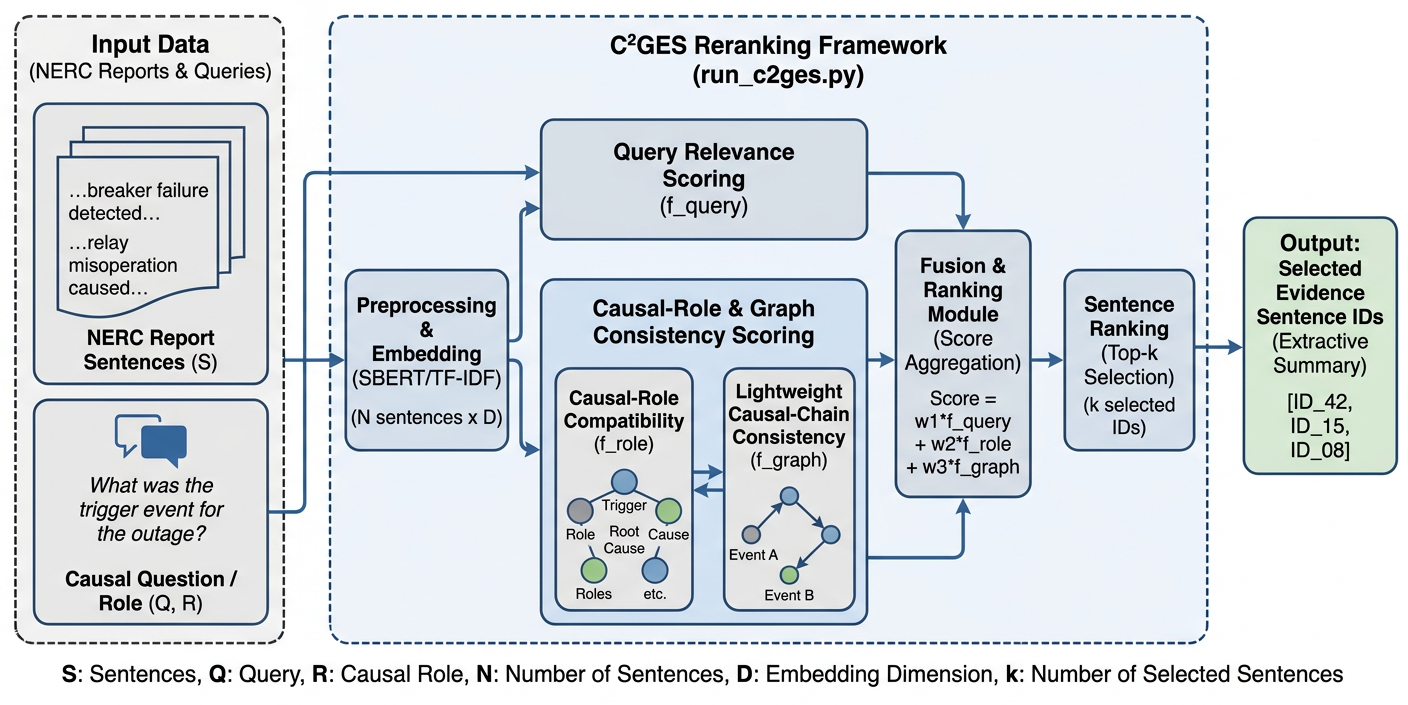
\includegraphics[width=\textwidth]{charts/architecture_diagram_1.png}
\caption{Architecture Overview}
\label{fig:architecture_overview}
\end{figure*}

\begin{figure*}[t]
\centering
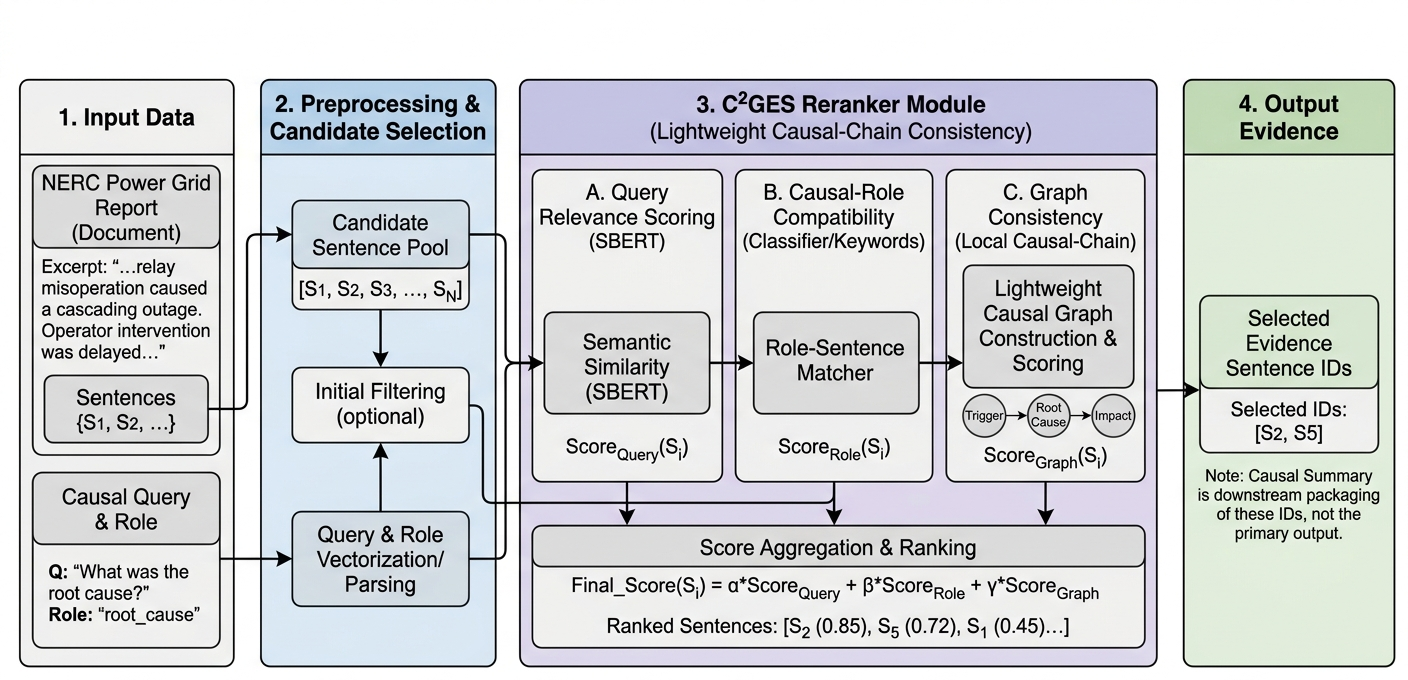
\includegraphics[width=\textwidth]{charts/pipeline_overview_2.png}
\caption{Pipeline Overview}
\label{fig:pipeline_overview}
\end{figure*}

The C\textsuperscript{2}GES procedure is deterministic once the document, question, role, prediction budget, and scoring weights are fixed. For each sentence, it computes the three scores, forms the weighted sum, sorts all candidate sentences, and returns the top \(K\) indices. The implementation path used for the experiments is \path{verification_pilot/scripts/run_c2ges.py}, and the Executor wrapper records the selected protocol and completed outputs under the experiment artifact path described in the benchmark section. The following pseudocode states the procedure at the level used in the pilot script.

\begin{algorithm}[t]
\caption{C\textsuperscript{2}GES evidence sentence reranking}
\begin{algorithmic}[1]
\REQUIRE Document sentences $D=\{s_1,\ldots,s_n\}$, question $q$, role $r$, budget $K$, weights $\theta=(w_q,w_r,w_g)$
\FOR{each sentence $s_j \in D$}
    \STATE Compute query relevance $Q_j = Q(s_j, q)$
    \STATE Compute role compatibility $R_j = R(s_j, r)$
    \IF{$r \in \{\text{propagation/response}, \text{mitigation}\}$}
        \STATE Compute chain consistency $G_j = G(s_j, D, r)$
    \ELSE
        \STATE Set $G_j = 0$
    \ENDIF
    \STATE Compute $S_j = w_q Q_j + w_r R_j + w_g G_j$
\ENDFOR
\STATE Sort sentence IDs $j$ by descending $S_j$, using document order for ties
\RETURN top-$K$ sentence IDs
\end{algorithmic}
\end{algorithm}

The computational cost is limited because the method reranks sentences within a single report or excerpt. If a document contains \(n\) sentences and text features have effective dimension \(d\), computing query relevance with sparse vectors costs \(O(nd)\) in the worst case but is lower under sparse indexing. Role compatibility costs \(O(nm)\), where \(m\) is the number of role and domain cue features. A naive chain-consistency computation over all sentence pairs costs \(O(n^2|\mathcal{R}|)\), but a local context window reduces the cost to \(O(nh|\mathcal{R}|)\), where \(h\) is the window radius recorded in the implementation configuration. Sorting costs \(O(n\log n)\), and the top-\(K\) selection can be implemented as \(O(n\log K)\) if needed. Since the benchmark contains 40 reports or excerpts and 200 role-conditioned questions, this lightweight design is appropriate for reproducible evaluation without requiring large-scale neural training.

The key design choice is the additive score decomposition with a role-selective graph gate. A more complex architecture could learn latent interactions among query, role, and document graph features, but the benchmark size and label provenance favor a transparent reranker whose ablation behavior can be inspected directly. In contrast to prior graph summarization methods that train heterogeneous or multiplex graph neural networks \cite{wang2020heterogeneous}, \cite{jing2021multiplex}, C\textsuperscript{2}GES uses graph information as a small consistency signal over candidate sentences. This keeps the method aligned with the central research question: whether causal-role-aware scoring improves sentence-ID evidence recovery for public power-grid maintenance, reliability, disturbance, and lessons-learned report text.

\section{Experiments}

\label{sec:experiments}

\subsection{Setup and Data}

\label{sec:setup_and_data}

The experiments evaluate whether C\textsuperscript{2}GES improves role-conditioned evidence sentence selection over generic retrieval and extractive summarization baselines. The evaluated benchmark is the local agent-verified candidate dataset at \path{verification_pilot/agent_audit_40doc/}, containing 40 public NERC reports or report excerpts, 200 causal questions, and 608 evidence sentence IDs. Each document contributes five role-conditioned questions, one for each role: trigger event, root cause, propagation or response, impact, and mitigation. Schema and evidence validation reported 0 errors, so the evaluation uses the provided sentence IDs directly. The labels are agent-rewritten and agent-verified candidate labels, and the experiment measures agreement with those candidate evidence annotations.

The evaluation unit is a document-role question. For each example \((D_i,q_{i,r},r)\), every method returns \(K=3\) predicted evidence sentence IDs. The primary comparison uses held-out predictions from the Executor artifact, with document-level 5-fold selection for C\textsuperscript{2}GES weight and protocol choices. Fold assignment is deterministic by \texttt{sha256(doc\_id) modulo 5}, which keeps all questions from the same document in the same fold and prevents document-level leakage across selection and held-out evaluation. The final experiment package was executed once; uncertainty estimates come from document-cluster bootstrap resampling and aggregate variation across evaluation examples, not from multiple random seeds or repeated independent runs. The Executor produced one held-out aggregate per condition, and the tables report the provided aggregate mean and standard-deviation fields from that completed run artifact.

The main conditions are limited to the controlled retrieval and ranking methods used in the benchmark. Positional selection returns the leading sentences and tests whether evidence is concentrated near the start of report excerpts. TF-IDF query retrieval ranks sentences by lexical similarity to the role-conditioned question, while TF-IDF centroid ranks sentences by similarity to the document centroid and therefore represents generic salience. TextRank and LexRank provide graph-centrality summarization baselines, using sentence similarity structure rather than role-specific evidence supervision \cite{khor2021text}, \cite{belwal2020graphbased}, \cite{setiawan2025impact}. The causal cue ranker prioritizes sentences with causal trigger language. SBERT query retrieval represents semantic matching with dense sentence embeddings, following the use of BERT-style sentence representations in extractive summarization and retrieval \cite{abdelsalam2022performance}, \cite{feng2022languageagnostic}. C\textsuperscript{2}GES is the proposed role-aware reranker. A scoped post-freeze supplement additionally evaluates deterministic Okapi BM25 query retrieval on the same sentence pools and role-conditioned questions, using lowercase regex tokenization with \(k_1=1.5\) and \(b=0.75\), without changing labels, segmentation, C\textsuperscript{2}GES weights, or the primary \(K=3\) protocol.

The ablation suite isolates the scoring terms in C\textsuperscript{2}GES. The query-only ablation retains the query relevance term and removes both role compatibility and chain consistency. The no-role ablation removes \(R(s,r)\) while preserving query and chain features, testing whether the causal role signal is responsible for the improvement. The no-graph ablation removes \(G(s,D,r)\), testing whether the role-selective causal-chain consistency term changes aggregate evidence recovery. A fixed legacy version of the full C\textsuperscript{2}GES scorer is retained as a comparison for the revised selection protocol, but the main method remains the full role-selective C\textsuperscript{2}GES reranker.

Three protocol-matched learned and LLM baselines extend the comparison beyond deterministic methods, executed with the prepared harness in the released code package on the same 200 questions, the same sentence pools, the same \(K=3\) budget, and the same evaluation metrics: (i) a neural cross-encoder reranker (\texttt{cross-encoder/ms-marco-MiniLM-L-6-v2}) that scores each question-sentence pair directly; (ii) a BGE reranker (\texttt{BAAI/bge-reranker-base}); and (iii) a zero-shot LLM selector (\texttt{deepseek-chat}, temperature 0, one API call per question) that receives the role question and the full sentence-ID list of the document and returns exactly three evidence sentence IDs. Both neural rerankers ran locally on CPU; the LLM baseline used a remote API endpoint. All 200 questions returned valid \(K=3\) predictions in every run. Paired statistics against full C\textsuperscript{2}GES use the same document-cluster bootstrap protocol (10000 samples) applied per-question against the Executor run's \texttt{details.jsonl}.

\subsection{Hyperparameters and Reproducibility}

\label{sec:hyperparameters_and_reproducibility}

Table 2 gives the experimental settings using short method abbreviations. The abbreviation mapping is included below the table so that table cells remain compact while the text preserves descriptive method names. The final C\textsuperscript{2}GES condition uses the selected role-gated-chain configuration recorded in \texttt{cv\_protocol.json}: \(w_q=0.52\), \(w_r=0.40\), \(w_g=0.08\), with graph active only for propagation/response and mitigation. The prediction budget is \(K=3\), and tie-breaking follows stable document order after descending score. Sentence segmentation, feature construction, and baseline candidate pools are shared across conditions so that differences reflect ranking behavior rather than incompatible preprocessing. TF-IDF baselines use the same sentence and question text normalization as the C\textsuperscript{2}GES lexical query component, and graph-centrality baselines use the same sentence pool as the evidence-ID evaluation. The SBERT baseline is recorded as the semantic-query condition in the Executor artifact; model checkpoint details are part of the reproducibility package rather than a separate experimental result.

\begin{table}[ht]
\centering
\caption{Hyperparameter settings}
\label{tab:2}
\resizebox{\columnwidth}{!}{%
\begin{tabular}{ll}
\toprule
\textbf{Setting} & \textbf{Value} \\
\midrule
Task & Role-conditioned evidence-ID selection \\
Dataset & 40 docs, 200 qs \\
Evidence IDs & 608 \\
Roles/doc & 5 \\
Budget & \(K=3\) \\
Split & Doc-level 5-fold \\
Fold rule & SHA256 mod 5 \\
Primary metric & Evidence F1 \\
Main methods & Lead, TFQ, TFC, TNR, LXR, CTR, SBQ, C2G \\
Ablations & QOnly, NoRole, NoGraph, C2G \\
Selected weights & \(w_q=0.52, w_r=0.40, w_g=0.08\) \\
Graph-active roles & Propagation/response, mitigation \\
Label status & Agent-verified candidate \\
Execution count & 1 \\
Hardware & RTX A6000, CUDA \\
VRAM & 49140 MB \\
\bottomrule
\end{tabular}
}
\end{table}

\textit{Abbreviations: Lead = leading-sentence positional selector; TFQ = TF-IDF query retrieval; TFC = TF-IDF centroid salience; TNR = TextRank with NetworkX; LXR = LexRank; CTR = causal trigger ranker; SBQ = SBERT query retrieval; C2G = table abbreviation for the full C\textsuperscript{2}GES reranker; QOnly = C\textsuperscript{2}GES query-only ablation; NoRole = C\textsuperscript{2}GES without role compatibility; NoGraph = C\textsuperscript{2}GES without chain consistency.}

The selected C\textsuperscript{2}GES scorer is implemented by the post-freeze role-selective graph-gate runner under \path{post_freeze_revisions/role_selective_graph_gate/code/main.py}, while the validated pilot scripts remain the baseline for sentence segmentation, baseline ranking, and legacy C\textsuperscript{2}GES behavior. The experiment package records command lines, dataset paths, output paths, and label-provenance caveats in \path{metadata.json}; held-out predictions are stored in \path{heldout_predictions.jsonl}; and fold assignment plus selected configuration metadata are stored in \path{cv_protocol.json}. The completed quantitative source for the tables is the valid run artifact that contains non-null metric values. Placeholder files with null result fields are excluded from the paper's quantitative claims, preventing failed or incomplete bookkeeping artifacts from being treated as experimental outcomes.

The hyperparameters were kept small and interpretable. The candidate grid contains seven lightweight configurations combining additive-chain, role-gated-chain, and fixed legacy scoring families; selection is performed within the document-level 5-fold protocol rather than by hand-tuning on the final aggregate table. The prediction budget is \(K=3\), matching the evidence sentence selection objective and keeping precision meaningful. The C\textsuperscript{2}GES score uses the three-term decomposition in Section 4, and ablations are implemented by setting the corresponding component weight to zero. Baseline implementations use the same sentence segmentation and candidate sentence pool as C\textsuperscript{2}GES, so differences reflect ranking behavior rather than preprocessing differences. This shared candidate pool is important because the benchmark evaluates sentence IDs directly; a method that selects a near-equivalent text span with a shifted sentence boundary is still penalized under the evidence-ID metric.

Runtime and hardware are reported for reproducibility, not as a research contribution. Experiments were executed in an environment with CUDA GPU availability on an NVIDIA RTX A6000 with 49140 MB of VRAM. The evaluated methods are lightweight sentence rankers over 40 reports or excerpts, so the computational bottleneck is feature extraction and sentence scoring rather than large model training. This setup makes the benchmark practical to rerun and supports direct inspection of predictions, ablations, and role-conditioned errors.

\subsection{Metrics and Statistical Testing}

\label{sec:metrics_and_statistical_testing}

The evaluation metrics are defined before reporting results because the task is set prediction rather than summary generation. For each example, let \(\hat{Y}\) be the predicted top-\(K\) sentence-ID set and \(Y\) be the candidate evidence set. Evidence precision is
\[
P=\frac{|\hat{Y}\cap Y|}{|\hat{Y}|},
\]
with higher values indicating that selected sentences are more frequently annotated as evidence. Evidence recall is
\[
R=\frac{|\hat{Y}\cap Y|}{|Y|},
\]
with higher values indicating that the method recovers more of the annotated evidence. The primary metric, evidence F1, is the harmonic mean
\[
F_1=\frac{2PR}{P+R},
\]
defined as 0 when both \(P\) and \(R\) are 0. It ranges from 0 to 1, where higher is better, and has no physical unit.

ROUGE-L over selected evidence text is a secondary text-overlap metric. For each example, the predicted sentence texts are concatenated and compared with the concatenated candidate evidence sentence texts using the longest common subsequence formulation of ROUGE-L. Its range is 0 to 1, higher is better, and it measures surface overlap rather than causal adequacy. The main graph and role claims are therefore based on evidence-ID precision, recall, F1, and paired evidence-F1 comparisons; ROUGE-L is used only to check whether better sentence-ID recovery is accompanied by stronger surface overlap. Role coverage is used as a diagnostic to determine whether retrieved evidence spans the five causal roles, while ablation deltas measure the difference in evidence F1 between full C\textsuperscript{2}GES and each component-removed variant. Qualitative case studies inspect selected and annotated sentence IDs to identify role-mismatch, neighboring-sentence, and implicit-cause errors.

The statistical analysis uses paired comparisons over the same evaluation examples. The predefined primary comparison is full C\textsuperscript{2}GES against TF-IDF query retrieval on evidence F1, because TF-IDF query retrieval is the strongest lexical retrieval baseline and directly tests whether role-aware reranking adds value beyond question matching. Secondary paired comparisons evaluate C\textsuperscript{2}GES against SBERT query retrieval, query-only C\textsuperscript{2}GES, no-role C\textsuperscript{2}GES, no-graph C\textsuperscript{2}GES, and the fixed legacy C\textsuperscript{2}GES scorer. The Results section reports document-cluster paired bootstrap mean differences, 95\% confidence intervals, and bootstrap p-values from the Executor artifact. The bootstrap resamples the 40 documents, not the 200 role questions, because questions from the same document share report context, sentence pools, and annotation history. No seed-wise t-tests are reported, and the non-primary p-values are treated as diagnostic evidence rather than as additional primary hypothesis tests.

\section{Results}

\label{sec:results}

\subsection{Main Quantitative Results}

\label{sec:main_quantitative_results}

The aggregate results show that the full C\textsuperscript{2}GES reranker is the strongest condition across all reported metrics among the main deterministic retrieval and ranking methods (the learned and LLM baselines are reported separately in Section~\ref{sec:learned_llm_baselines}). Table 3 reports mean and standard deviation across evaluation examples from the completed Executor run, with BM25 added by the scoped post-freeze supplement; these standard-deviation fields are not confidence intervals. The full C\textsuperscript{2}GES evidence F1 exceeds TF-IDF query retrieval, BM25 query retrieval, and SBERT query retrieval, indicating that causal-role-aware reranking improves beyond both lexical and dense semantic question matching. The same pattern appears in precision and recall, where C\textsuperscript{2}GES improves precision while also retrieving more annotated evidence, so the F1 gain is not driven by a one-sided precision-recall tradeoff. Building on this observation, the selected-evidence ROUGE-L result also increases over TF-IDF, BM25, and SBERT query retrieval, showing that better sentence-ID recovery is accompanied by stronger surface overlap with the annotated evidence text.

\begin{table*}[ht]
\centering
\caption{Performance comparison of different methods on Evidence F1, Precision, Recall, ROUGE-L}
\label{tab:3}
\begin{tabular}{lrrrr}
\toprule
\textbf{Method} & \textbf{Evidence F1} & \textbf{Precision} & \textbf{Recall} & \textbf{ROUGE-L} \\
\midrule
Lead sentence selector & 0.0545 $\pm$ 0.1426 & 0.0533 $\pm$ 0.1392 & 0.0592 $\pm$ 0.1634 & 0.1822 $\pm$ 0.1233 \\
TF-IDF query retrieval & 0.2122 $\pm$ 0.2293 & 0.2050 $\pm$ 0.2253 & 0.2471 $\pm$ 0.2976 & 0.3224 $\pm$ 0.1931 \\
BM25 query retrieval & 0.2273 $\pm$ 0.2410 & 0.2217 $\pm$ 0.2410 & 0.2575 $\pm$ 0.2971 & 0.3247 $\pm$ 0.1929 \\
TF-IDF centroid salience & 0.0688 $\pm$ 0.1556 & 0.0717 $\pm$ 0.1594 & 0.0717 $\pm$ 0.1772 & 0.2090 $\pm$ 0.1360 \\
TextRank with NetworkX & 0.0700 $\pm$ 0.1549 & 0.0733 $\pm$ 0.1604 & 0.0725 $\pm$ 0.1757 & 0.2126 $\pm$ 0.1297 \\
LexRank & 0.0167 $\pm$ 0.0946 & 0.0183 $\pm$ 0.1011 & 0.0154 $\pm$ 0.0902 & 0.1438 $\pm$ 0.0810 \\
Causal trigger ranker & 0.1071 $\pm$ 0.1986 & 0.1067 $\pm$ 0.1993 & 0.1242 $\pm$ 0.2537 & 0.2302 $\pm$ 0.1569 \\
SBERT query retrieval & 0.1972 $\pm$ 0.2301 & 0.1883 $\pm$ 0.2200 & 0.2329 $\pm$ 0.3037 & 0.3067 $\pm$ 0.1884 \\
Full C\textsuperscript{2}GES reranker & \textbf{0.2983 $\pm$ 0.2409} & \textbf{0.2950 $\pm$ 0.2454} & \textbf{0.3325 $\pm$ 0.2993} & \textbf{0.3732 $\pm$ 0.1933} \\
\bottomrule
\end{tabular}
\end{table*}

The Executor artifact does not define easy and hard regimes, so the paper does not infer regime-specific results. The all-regime aggregate still answers the primary benchmark question because every method is compared over the same 200 document-role questions. The supplemental BM25 result is stronger than TF-IDF query retrieval but remains below the full role-aware reranker at \(K=3\). As shown in Fig.~\ref{fig:evidence_f1_across_main_retrie}, the original main-condition chart separates the full C\textsuperscript{2}GES reranker from the non-BM25 lexical and semantic query baselines, while position-based and centrality-based summarizers recover less role-specific evidence. This makes ablation analysis, the BM25 supplement, and document-cluster paired bootstrap the main evidence for mechanism and statistical reliability.

\begin{figure}[t]
\centering
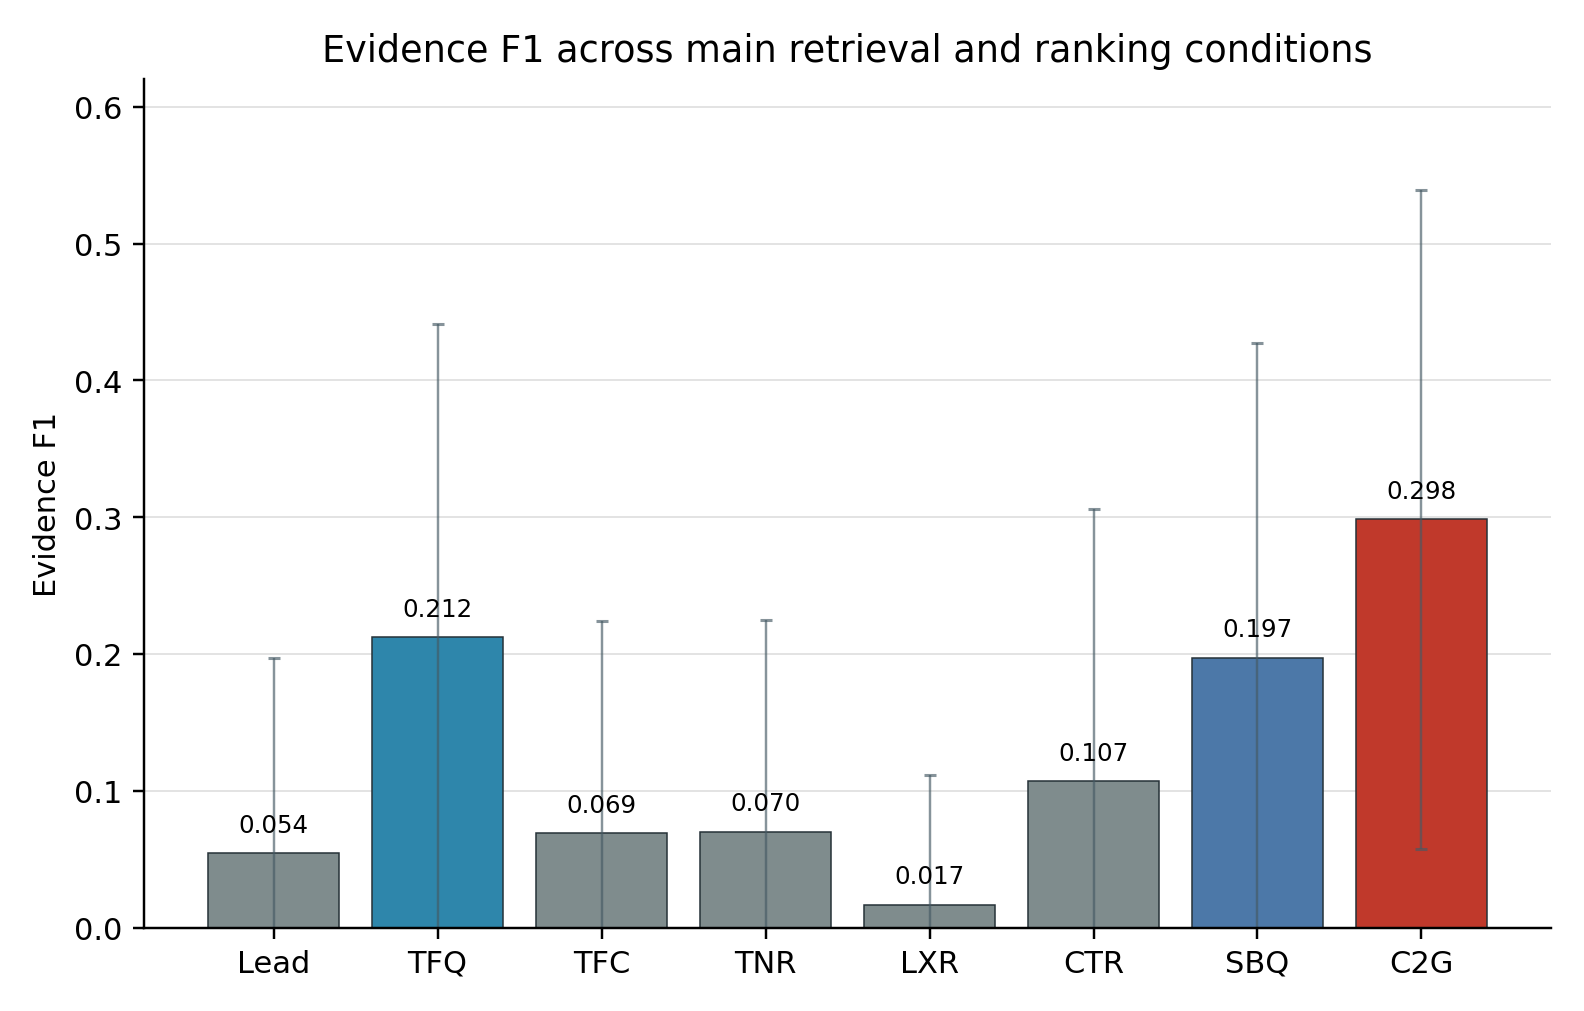
\includegraphics[width=0.95\columnwidth]{charts/fig_2.png}
\caption{Evidence F1 across main retrieval and ranking conditions}
\label{fig:evidence_f1_across_main_retrie}
\end{figure}

\begin{table*}[t]
\centering
\caption{Per-role full C\textsuperscript{2}GES evidence metrics and role-aware deltas}
\label{tab:per_role_full_metrics}
\resizebox{\textwidth}{!}{%
\begin{tabular}{lrrrrr}
\toprule
\textbf{Role} & \textbf{F1} & \textbf{Precision} & \textbf{Recall} & \textbf{F1 delta vs. TF-IDF query} & \textbf{F1 delta vs. NoRole} \\
\midrule
Trigger event & 0.3114 & 0.2833 & 0.4000 & +0.1006 & +0.0723 \\
Root cause & 0.2594 & 0.2500 & 0.2896 & +0.0470 & +0.0475 \\
Propagation/response & 0.2611 & 0.2750 & 0.2625 & +0.0436 & +0.0281 \\
Impact & 0.3429 & 0.3500 & 0.3625 & +0.1438 & +0.0988 \\
Mitigation & 0.3167 & 0.3167 & 0.3479 & +0.0955 & +0.0971 \\
\bottomrule
\end{tabular}
}
\end{table*}

Table~\ref{tab:per_role_full_metrics} shows that the aggregate gain is not confined to one role. Impact evidence has the highest F1, consistent with the fact that impact sentences often contain measurable quantities such as MW reductions, load shed, or customer effects. Root-cause and propagation/response questions remain harder because the correct evidence can be close to neighboring causal context but still require selecting a specific equipment, protection, or response sentence. The deltas against TF-IDF query retrieval are positive for all five roles, while the deltas against the no-role ablation show that role compatibility contributes most visibly for impact, mitigation, and trigger-event evidence.

\begin{table}[ht]
\centering
\caption{Role-stratified evidence F1 at \(K=3\) for the strongest lexical baseline, the no-role ablation, and the full reranker (all values from the supplement artifact)}
\label{tab:role_strata_baselines}
\resizebox{\columnwidth}{!}{%
\begin{tabular}{lrrrr}
\toprule
\textbf{Role} & \textbf{BM25 query} & \textbf{NoRole} & \textbf{Full C\textsuperscript{2}GES} & \textbf{Full $-$ BM25} \\
\midrule
Trigger event & 0.2250 & 0.2392 & \textbf{0.3114} & +0.0864 \\
Root cause & 0.2154 & 0.2119 & \textbf{0.2594} & +0.0440 \\
Propagation/response & 0.2289 & 0.2330 & \textbf{0.2611} & +0.0321 \\
Impact & 0.2181 & 0.2440 & \textbf{0.3429} & +0.1248 \\
Mitigation & 0.2490 & 0.2195 & \textbf{0.3167} & +0.0676 \\
\bottomrule
\end{tabular}
}
\end{table}

Table~\ref{tab:role_strata_baselines} extends the role stratification to the strongest supplemental lexical baseline. Full C\textsuperscript{2}GES beats BM25 query retrieval on every role, but the margin is far from uniform: it is largest for impact (+0.1248) and trigger event (+0.0864), where role-specific surface signals such as measured quantities and event-start language are most discriminative, and smallest for propagation/response (+0.0321) and root cause (+0.0440), where the correct evidence is lexically close to neighboring causal context. The no-role ablation column sharpens this reading: removing role compatibility collapses the reranker roughly to baseline level on every role, and for mitigation (0.2195) and root cause (0.2119) the no-role variant actually falls below BM25 (0.2490 and 0.2154), so the role term is not merely additive noise on top of query relevance but the component that carries the roles where the full method gains most (impact, mitigation, trigger event; compare the NoRole deltas in Table~\ref{tab:per_role_full_metrics}). Propagation/response is the weakest role for role conditioning under both comparisons, which is consistent with the role-selective graph gate being targeted at exactly the roles where lexical role cues are least sufficient.

Cross-document heterogeneity is substantial and is reported here as an honest robustness observation rather than smoothed away. The standard deviations in Table~\ref{tab:3} are computed over the 200 question-level scores and are of the same order as the means (about 0.24 against a mean of 0.2983 for the full reranker), which is expected for a strict top-\(K\) set-overlap metric scored per question. Aggregating to the document level, per-document mean evidence F1 for full C\textsuperscript{2}GES ranges from 0.0800 to 0.5219 across the 40 documents (mean 0.2983, sample standard deviation 0.1092), with no document at zero; BM25 query retrieval spans 0.0571 to 0.5000, and SBERT query retrieval leaves one document with no recovered evidence at all. Because documents, not questions, are the natural unit of this heterogeneity, all interval estimates in this paper use document-cluster bootstrap resampling rather than question-level resampling.

\subsection{Paired Comparisons and Ablations}

\label{sec:paired_comparisons_and_ablations}

The paired comparisons confirm that C\textsuperscript{2}GES's advantage is strongest against query-only retrieval and role-removed variants. Table 4 summarizes document-cluster paired bootstrap comparisons for evidence F1. The difference against TF-IDF query retrieval supports the pre-specified primary comparison, while the remaining comparisons are diagnostic. The comparison against SBERT query retrieval supports the same qualitative conclusion for semantic matching. The comparison against the no-role ablation identifies role compatibility as a major source of the aggregate improvement. The comparison against the no-graph ablation is much smaller, but the role-selective gate produces a positive auxiliary graph/chain gain under document-cluster bootstrap. For transparency, the role-selective gate itself originated in a post-freeze revision: an earlier frozen configuration applied the graph term to all five roles and showed no reliable graph benefit, and the gated variant reported here was selected afterwards within the document-level 5-fold candidate protocol, so its \(p=0.0254\) should be read as diagnostic support for a small auxiliary effect rather than as a confirmatory pre-registered test.

\begin{table*}[ht]
\centering
\caption{Document-cluster paired bootstrap comparisons for evidence F1}
\label{tab:4}
\resizebox{\textwidth}{!}{%
\begin{tabular}{lrrrl}
\toprule
\textbf{Comparison} & \textbf{Mean evidence-F1 diff} & \textbf{Document-cluster 95\% CI} & \textbf{p-value} & \textbf{Interpretation} \\
\midrule
Full C\textsuperscript{2}GES vs. TF-IDF query retrieval & 0.0861 & [0.0581, 0.1145] & <0.001 & Primary gain over lexical query retrieval \\
Full C\textsuperscript{2}GES vs. BM25 query retrieval & 0.0710 & [0.0423, 0.1000] & <0.001 & Supplemental gain over BM25 lexical retrieval \\
Full C\textsuperscript{2}GES vs. SBERT query retrieval & 0.1010 & [0.0629, 0.1388] & <0.001 & Diagnostic gain over semantic query retrieval \\
Full C\textsuperscript{2}GES vs. C\textsuperscript{2}GES query-only & 0.0831 & [0.0541, 0.1120] & <0.001 & Role and structure terms improve query-only ranking \\
Full C\textsuperscript{2}GES vs. C\textsuperscript{2}GES without role compatibility & 0.0688 & [0.0416, 0.0972] & <0.001 & Role compatibility is important \\
Full C\textsuperscript{2}GES vs. C\textsuperscript{2}GES without graph consistency & 0.0060 & [0.0014, 0.0119] & 0.0254 & Small role-selective graph gain \\
Full C\textsuperscript{2}GES vs. fixed legacy C\textsuperscript{2}GES & 0.0403 & [0.0178, 0.0621] & <0.001 & Revised protocol improves over fixed legacy scoring \\
\bottomrule
\end{tabular}
}
\end{table*}

\begin{table}[ht]
\centering
\caption{Supplemental \(K\)-sensitivity evidence F1}
\label{tab:k_sensitivity}
\resizebox{\columnwidth}{!}{%
\begin{tabular}{lrrr}
\toprule
\textbf{Method} & \(\mathbf{K=1}\) & \(\mathbf{K=3}\) & \(\mathbf{K=5}\) \\
\midrule
TF-IDF query retrieval & 0.1783 & 0.2122 & 0.2162 \\
BM25 query retrieval & 0.1857 & 0.2273 & 0.2208 \\
SBERT query retrieval & 0.1560 & 0.1972 & 0.2042 \\
Full C\textsuperscript{2}GES reranker & \textbf{0.2133} & \textbf{0.2983} & \textbf{0.2850} \\
\bottomrule
\end{tabular}
}
\end{table}

Table~\ref{tab:k_sensitivity} reports a bounded \(K\)-sensitivity check for the fixed final scorer and key retrieval baselines. The primary benchmark budget remains \(K=3\); the additional \(K=1\) and \(K=5\) rows are not used to select a new operating point. The C\textsuperscript{2}GES advantage is largest and statistically supported at \(K=3\), where the document-cluster bootstrap gain over BM25 is \(+0.0710\) evidence F1 with 95\% CI \([0.0423,0.1000]\). At \(K=5\), C\textsuperscript{2}GES remains ahead of BM25 by \(+0.0643\) evidence F1 with 95\% CI \([0.0331,0.0961]\). At \(K=1\), C\textsuperscript{2}GES has the highest aggregate F1, but its paired gains over TF-IDF and BM25 have confidence intervals that cross zero, so the stricter one-sentence setting should be interpreted as suggestive rather than conclusive.

The supplement artifact additionally records paired document-cluster bootstrap comparisons against the semantic baseline at every budget, and these are reported here for completeness. The gain over SBERT query retrieval is \(+0.0573\) evidence F1 (95\% CI \([0.0093, 0.1013]\), \(p=0.0182\)) at \(K=1\) and \(+0.0808\) (\([0.0387, 0.1208]\), \(p<0.001\)) at \(K=5\); at \(K=5\) the gain over TF-IDF query retrieval is \(+0.0688\) (\([0.0421, 0.0949]\), \(p<0.001\)). At the primary \(K=3\) budget, the SBERT comparison is significant not only for F1 but also for evidence precision (\(+0.1067\), \([0.0683, 0.1467]\)) and evidence recall (\(+0.0996\), \([0.0575, 0.1408]\)). These additional contrasts come from a single run artifact and are not corrected for multiple comparisons; only the TF-IDF comparison at \(K=3\) retains pre-specified primary status, and the \(K=1\) SBERT result in particular should be read as diagnostic, since it would not survive a conservative correction over the nine baseline comparisons in the artifact.

\begin{table}[ht]
\centering
\caption{Role-stratified evidence-F1 effect of role-selective graph consistency}
\label{tab:role_graph_delta}
\resizebox{\columnwidth}{!}{%
\begin{tabular}{lrrr}
\toprule
\textbf{Role} & \textbf{Full C\textsuperscript{2}GES} & \textbf{NoGraph} & \textbf{Delta} \\
\midrule
Trigger event & 0.3114 & 0.3114 & 0.0000 \\
Root cause & 0.2594 & 0.2594 & 0.0000 \\
Propagation/response & 0.2611 & 0.2527 & +0.0083 \\
Impact & 0.3429 & 0.3429 & 0.0000 \\
Mitigation & 0.3167 & 0.2952 & +0.0214 \\
\bottomrule
\end{tabular}
}
\end{table}

\begin{figure}[t]
\centering
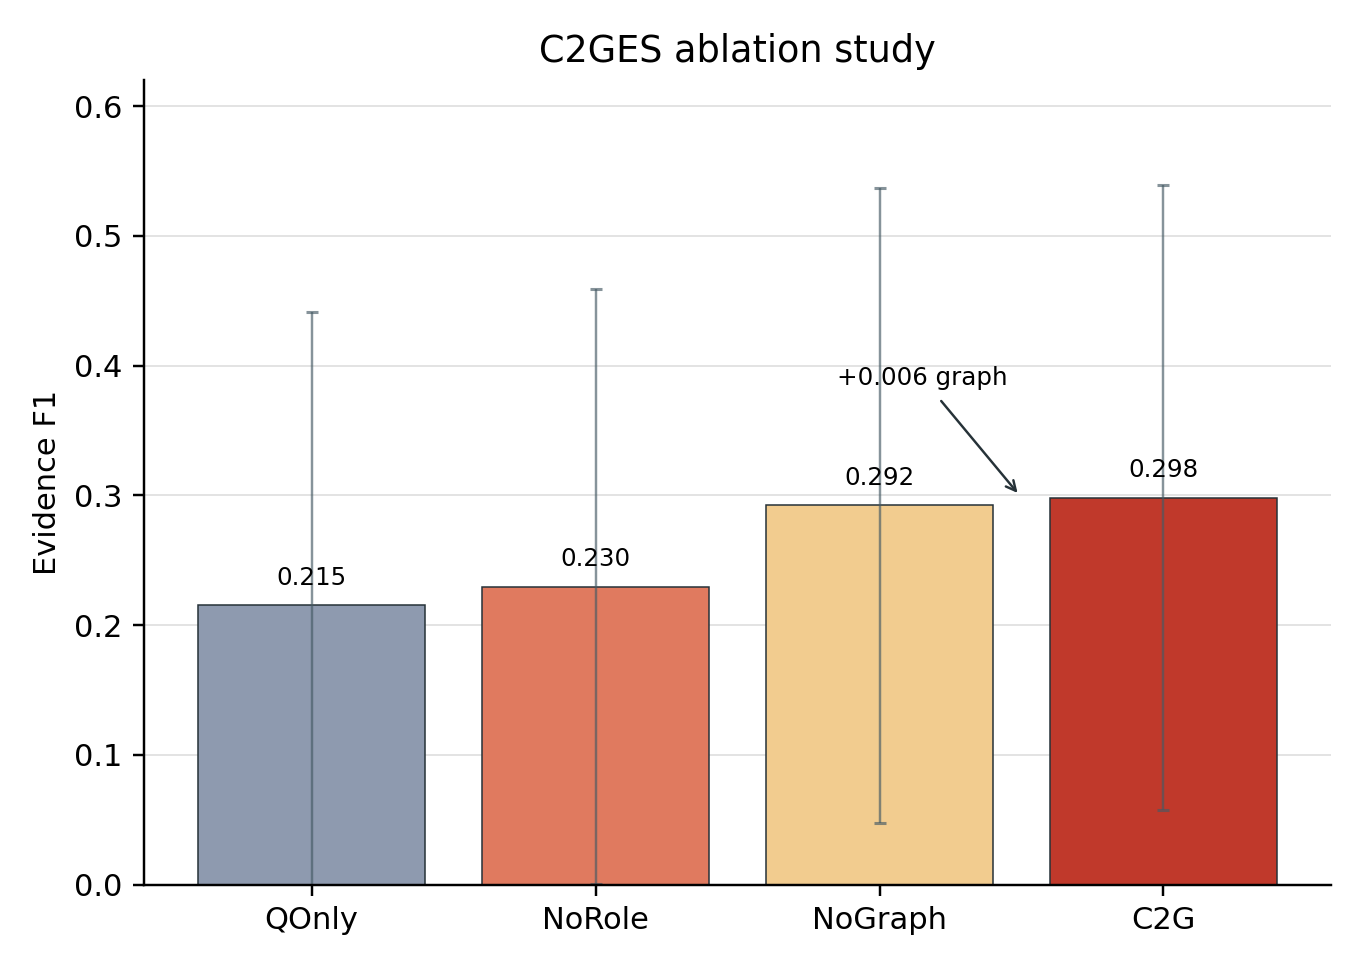
\includegraphics[width=0.95\columnwidth]{charts/fig_4.png}
\caption{C\textsuperscript{2}GES ablation study}
\label{fig:c_ges_ablation_study}
\end{figure}

The ablation results refine the main claim by separating role awareness from graph enhancement. Query-only C\textsuperscript{2}GES reaches 0.2152 evidence F1, close to TF-IDF query retrieval, which means the query component alone behaves like a relevance ranker. Removing role compatibility gives 0.2295 evidence F1, while removing graph consistency gives 0.2923 evidence F1. This ordering, also summarized in Fig.~\ref{fig:c_ges_ablation_study}, indicates that causal-role compatibility is the dominant mechanism behind improved evidence selection. The graph consistency term is included as a lightweight role-selective auxiliary feature, producing a small aggregate gain of 0.0060 evidence F1 over the no-graph variant.

Overall, the results support the first hypothesis in its central form. Full C\textsuperscript{2}GES improves over TF-IDF query retrieval, SBERT query retrieval, and the lead baseline on the same 200 document-role questions. The ablation evidence also supports the role-aware part of the hypothesis because removing role compatibility causes a large drop relative to the full reranker. The graph-related claim is narrower but positive: role-selective chain consistency adds a small auxiliary improvement, and Table~\ref{tab:role_graph_delta} shows that the effect is concentrated in propagation/response and mitigation. Building on this observation, the discussion interprets C\textsuperscript{2}GES as a role-aware evidence reranker with a lightweight structural auxiliary term rather than as a graph-driven causal inference model.

\subsection{Learned and LLM Baselines}

\label{sec:learned_llm_baselines}

Table~\ref{tab:learned_llm_baselines} reports the three protocol-matched learned and LLM baselines alongside the key existing conditions, with paired document-cluster bootstrap differences against the full C\textsuperscript{2}GES reranker (delta defined as baseline minus C\textsuperscript{2}GES, so negative values favor C\textsuperscript{2}GES). Three findings follow, and each is stated with its statistical qualification.

\begin{table*}[ht]
\centering
\caption{Learned and LLM baselines under the paper's protocol (\(K=3\), 200 questions, same metrics), with paired document-cluster bootstrap comparison against full C\textsuperscript{2}GES (delta = baseline \(-\) C\textsuperscript{2}GES; 10000 samples)}
\label{tab:learned_llm_baselines}
\resizebox{\textwidth}{!}{%
\begin{tabular}{lrrrrrl}
\toprule
\textbf{Method} & \textbf{Evidence F1} & \textbf{Precision} & \textbf{Recall} & \textbf{ROUGE-L} & \textbf{F1 diff vs. full C\textsuperscript{2}GES [95\% CI]} & \textbf{p} \\
\midrule
SBERT query retrieval & 0.1972 & 0.1883 & 0.2329 & 0.3067 & \(-0.1010\) \([-0.1388, -0.0629]\) & <0.001 \\
TF-IDF query retrieval & 0.2122 & 0.2050 & 0.2471 & 0.3224 & \(-0.0861\) \([-0.1145, -0.0581]\) & <0.001 \\
BM25 query retrieval & 0.2273 & 0.2217 & 0.2575 & 0.3247 & \(-0.0710\) \([-0.1000, -0.0423]\) & <0.001 \\
BGE reranker (BAAI/bge-reranker-base) & 0.2604 & 0.2517 & 0.3013 & 0.3490 & \(-0.0379\) \([-0.0739, -0.0010]\) & 0.0448 \\
Cross-encoder (ms-marco-MiniLM-L-6-v2) & 0.2787 & 0.2717 & 0.3188 & 0.3667 & \(-0.0196\) \([-0.0539, +0.0140]\) & 0.246 \\
Full C\textsuperscript{2}GES reranker & 0.2983 & 0.2950 & 0.3325 & 0.3732 & --- & --- \\
LLM zero-shot (deepseek-chat, temp.\ 0) & \textbf{0.5887} & \textbf{0.5950} & \textbf{0.6342} & \textbf{0.5942} & \(+0.2905\) \([+0.2533, +0.3255]\) & <0.001 \\
\bottomrule
\end{tabular}
}
\end{table*}

First, within the transparent, deterministic, CPU-deployable reranker class, full C\textsuperscript{2}GES remains the strongest tested condition, but the two statements that make up this claim have different strengths and both are stated here. The BGE reranker is behind C\textsuperscript{2}GES by \(-0.0379\) evidence F1 with a document-cluster confidence interval whose upper endpoint barely excludes zero (\([-0.0739, -0.0010]\), \(p=0.0448\)): a borderline-significant deficit. The cross-encoder is behind by \(-0.0196\) with a confidence interval that clearly crosses zero (\([-0.0539, +0.0140]\), \(p=0.246\)): C\textsuperscript{2}GES is ahead in the point estimate, but the data do not establish a statistically significant advantage over the cross-encoder, and no such advantage is claimed. Both neural rerankers, in turn, beat the lexical and semantic query baselines significantly (cross-encoder vs.\ TF-IDF \(+0.0665\) \([0.0389, 0.0941]\), vs.\ SBERT \(+0.0815\) \([0.0544, 0.1069]\), both \(p<0.001\); BGE vs.\ TF-IDF \(+0.0482\) \([0.0210, 0.0747]\) \(p<0.001\), vs.\ SBERT \(+0.0632\) \([0.0260, 0.0995]\) \(p=0.0006\)), landing between BM25 and full C\textsuperscript{2}GES as expected for general-domain rerankers applied without domain adaptation.

Second, the zero-shot LLM selector decisively outperforms every non-LLM condition: 0.5887 evidence F1, a paired gain of \(+0.2905\) over full C\textsuperscript{2}GES (\([+0.2533, +0.3255]\), \(p<0.001\)), roughly doubling the deterministic reranker. This result is reported as a genuine upper reference, with two qualifications. The label-provenance caveat of Section~\ref{sec:cue_lexicon_construction_and_circularity} applies with particular force: the benchmark labels are LLM-agent-generated and LLM-agent-verified, so part of the LLM baseline's advantage may reflect LLM--LLM agreement rather than pure task superiority, and until the pre-announced human-gold subset exists, 0.5887 should be read as an upper bound under agent-verified candidate labels. At the same time, the LLM score carries an important positive message for the benchmark contribution itself: the labels are learnable, the task is far from saturated, and the benchmark discriminates across a 0.05--0.59 evidence-F1 range, which is exactly the headroom a method-development benchmark needs.

Third, the accuracy ordering must be read jointly with the deployment characteristics in Table~\ref{tab:deployment_tradeoff}, which is where the paper's transparency positioning now carries data rather than rhetoric. The LLM baseline required one API call per question against a remote proprietary endpoint (200 calls, roughly 8.5 minutes wall clock, about 2.5 seconds per question including a full-document prompt, and an estimated US\$0.2--0.3 for the full benchmark at published rates), returns no per-term score decomposition, and is exposed to provider-side model-version drift. The deterministic reranker and both neural rerankers run locally on CPU with zero marginal API cost, but only C\textsuperscript{2}GES decomposes every ranking decision into three inspectable terms with published constants and produces bit-for-bit reproducible rankings. The load-bearing distinction here is auditability rather than connectivity: a locally hosted open-weights LLM would also run offline, but would still return no per-term score decomposition and no reproducibility guarantee. For reliability post-event review --- where selected evidence may support regulatory or corrective-action claims and per-sentence selection may need to be audited or disputed --- per-term decomposability, determinism, and auditability are requirements rather than conveniences, with offline CPU operation and negligible cost as secondary practical benefits, and within the class of methods that satisfies these requirements, C\textsuperscript{2}GES remains the best tested option.

\begin{table*}[ht]
\centering
\caption{Deployment-class tradeoff between the deterministic reranker, neural rerankers, and zero-shot LLM selection (accuracy from Table~\ref{tab:learned_llm_baselines}; LLM cost and latency measured on the reported run)}
\label{tab:deployment_tradeoff}
\resizebox{\textwidth}{!}{%
\begin{tabular}{llll}
\toprule
\textbf{Property} & \textbf{Full C\textsuperscript{2}GES} & \textbf{Neural rerankers (CE / BGE)} & \textbf{Zero-shot LLM (deepseek-chat)} \\
\midrule
Evidence F1 (\(K=3\)) & 0.2983 & 0.2787 / 0.2604 & 0.5887 \\
Per-term score decomposition & Yes (three terms, published constants) & No (learned scoring, opaque weights) & No (no sentence-level scores) \\
Deterministic / reproducible & Bit-for-bit, no model dependence & Deterministic given a fixed checkpoint & Temperature 0, but subject to provider model-version drift \\
Offline / deployment & Offline, CPU, no model download & Offline, CPU-capable, checkpoint download & Remote proprietary API required \\
Marginal cost (full benchmark) & None & None (local inference) & \(\approx\)US\$0.2--0.3 (200 API calls) \\
Latency source & Sparse feature scoring & Local neural inference & \(\approx\)2.5 s/question network round trip (\(\approx\)8.5 min total) \\
\bottomrule
\end{tabular}
}
\end{table*}

\section{Qualitative Error Analysis}

\label{sec:qualitative_error_analysis}

Aggregate results show that role-aware reranking helps, but the example-level predictions reveal why the benchmark remains difficult. This section inspects held-out predictions from \texttt{details.jsonl}; the examples are illustrative and are not used for additional tuning. The purpose is to connect quantitative patterns to report-level behavior while keeping the main evidence in the aggregate tables and document-cluster paired comparisons.

One successful role-disambiguation case comes from \path{nerc_014_april_may_2018_solar_pv_disturbance_report::impact}. The question asks for measurable operational impacts involving Angeles Forest solar PV output, CAISO net load, and a combined-cycle unit. The labeled evidence IDs are \texttt{s051}, \texttt{s071}, and \texttt{s028}. Full C\textsuperscript{2}GES selects \texttt{s071}, \texttt{s051}, and \texttt{s013}, giving evidence F1 0.667, while TF-IDF query retrieval selects \texttt{s013}, \texttt{s079}, and \texttt{s020}, giving F1 0.0. The selected C\textsuperscript{2}GES evidence includes the sentences stating that the 500 kV line fault reduced BPS-connected solar PV output in CAISO and by 17 MW in LADWP, and that the net load increase was about 900 MW and 100 MW in the CAISO footprint. This case illustrates the main intended behavior: the role-aware score favors sentences with impact quantities and operational consequence language rather than retrieving sentences that share event vocabulary but do not answer the impact question.

A representative failure occurs in \path{nerc_009_odessa_disturbance_report::root_cause}. The question asks what equipment failure caused the initial transformer fault at the combined-cycle plant. The labeled evidence IDs are \texttt{s007} and \texttt{s008}, which state that a single-line-to-ground fault occurred on a generator step-up transformer and that the fault was caused by a failed surge arrester during startup for testing. Full C\textsuperscript{2}GES selects \texttt{s012}, \texttt{s062}, and \texttt{s070}, giving F1 0.0, while TF-IDF query retrieval selects \texttt{s007}, \texttt{s062}, and \texttt{s065}, giving F1 0.4. The C\textsuperscript{2}GES false positives are still topically related to the disturbance, including generation loss and plant protection language, but they miss the specific failed surge-arrester cause. This is a role-mismatch and neighboring-context error: the method recognizes causal and equipment-related context but selects sentences adjacent to the correct causal explanation rather than the labeled root-cause evidence itself.

A second failure pattern appears in \path{nerc_012_january_11_oscillation_event_report::trigger_event}. The question asks what event conditions marked the start of the Florida oscillation and activated cyclical turbine valve behavior. The candidate evidence set includes the time-line sentence about the oscillation observed around 08:11:16 UTC and the sentence describing PLI operation causing intercept valves to shut and reopen periodically. Full C\textsuperscript{2}GES selects broader executive-summary and oscillation-description sentences, while TF-IDF retrieves one of the trigger sentences. This shows that the current role cues can prefer general event descriptions over precise trigger-time evidence when the report contains repeated descriptions of the same disturbance.

The role-selective graph ablation is also visible at the prediction level. For trigger, root-cause, and impact questions, the revised full scorer intentionally matches the query-plus-role no-graph form; for example, in \path{nerc_001_november_13_wyoming_disturbance_report::impact}, both variants select \texttt{s022}, \texttt{s013}, and \texttt{s001}. The useful graph changes instead appear in the graph-active roles, where local chain context can move propagation/response or mitigation evidence into the top-\(K\) set. This behavior is consistent with the role-stratified results: graph consistency is a small auxiliary adjustment, not the main source of C\textsuperscript{2}GES's aggregate improvement.

These cases support three practical conclusions. First, role compatibility helps when the relevant evidence is marked by role-specific quantitative or causal language, as in the solar PV impact example. Second, false positives can remain semantically close to the correct evidence, which suggests that future work should improve sentence-boundary sensitivity, local context aggregation, and near-miss handling. Third, graph consistency is most defensible as a role-selective auxiliary signal for structurally contextual roles; stronger graph modeling remains future work.

\section{Discussion}

\label{sec:discussion}

The main finding is that role-aware evidence reranking is more effective than generic relevance retrieval for causal evidence selection in the evaluated NERC reports and report excerpts. Query-focused summarization work has established that the information need should condition content selection \cite{zhong2021qmsum}, and extractive summarization as text matching provides a strong baseline for sentence-level selection \cite{zhong2020extractive}. C\textsuperscript{2}GES extends this logic into a domain where the query is not merely topical but causal-role specific. The improvement over TF-IDF and SBERT query retrieval suggests that a sentence can be relevant to the same disturbance yet still fail to answer the requested role, which is exactly the distinction the benchmark was designed to expose.

The ablation pattern provides a technical insight: role compatibility matters more than the graph consistency term in the current implementation. This finding is consistent with graph-based summarization literature in a qualified way. Heterogeneous and multiplex graph summarizers can model rich structural relations when trained or parameterized for broad document summarization \cite{wang2020heterogeneous}, \cite{jing2021multiplex}, but C\textsuperscript{2}GES uses a lighter chain-consistency feature over a small role-conditioned benchmark. The role-selective revision shows that local causal-chain scoring can change top-\(K\) evidence selections for propagation/response and mitigation, but the aggregate gain remains small relative to the role-compatibility gain. This clarifies where the method's empirical force currently resides: the present contribution is role-aware evidence reranking with an auxiliary structural signal, not graph-driven causal inference.

The results also align with evidence-retrieval research that treats supporting text as the object of evaluation rather than as hidden context for a generated answer. Multi-step and hybrid evidence retrieval methods emphasize that downstream reasoning quality depends on retrieving the right support units \cite{liao2023muser}, \cite{liang2020hammer}. C\textsuperscript{2}GES applies that principle to public power-grid reports, where the evidence unit is a sentence ID and the information need is a causal-role question. This design is practically important because power-system analysts need traceable support for claims about causes, responses, and mitigations rather than fluent summaries that obscure provenance.

The power-grid setting makes the role distinction more than a linguistic preference. Cascading-failure and grid-reliability studies show that disturbances involve initiating events, propagation mechanisms, system responses, impacts, and corrective actions that must be interpreted together \cite{rajkumar2023cyber}, \cite{xie2022massively}. A generic summarizer may recover a salient outage statement, but an analyst asking about mitigation needs a different kind of evidence. C\textsuperscript{2}GES's stronger recall and precision indicate that role cues and report-local context help separate these functions in the candidate benchmark, supporting the premise that causal-role evidence selection is a meaningful intermediate task for grid maintenance and reliability report analysis.

The ablation interpretation of the method is intentionally narrower than causal counterfactual inference. Causal NLP work warns that causal language processing should distinguish textual prediction from stronger causal inference \cite{feder2022causal}. In this study, the diagnostic question is operational: what changes when the role or chain component is removed from the scorer? The answer is concrete. Removing role compatibility substantially reduces evidence recovery, while removing role-selective graph consistency causes a small but positive aggregate drop. This gives a diagnostic result for future method design: role modeling remains the primary investment, whereas graph structure should be developed as a bounded auxiliary mechanism unless stronger edge induction or role-transition learning produces larger evidence-selection gains.

The positioning of C\textsuperscript{2}GES relative to learned rerankers and LLM-based selection deserves an explicit statement, because zero-shot LLM rerankers now perform strongly on general retrieval benchmarks \cite{qin2024pairwise}, \cite{zhuang2024setwise}, \cite{ren2025selfcalibrated}. The value proposition of the deterministic reranker is not that it is expected to dominate such systems on evidence F1; it is per-term decomposability, determinism, and auditability, with offline CPU operation and low cost as secondary practical benefits. Every C\textsuperscript{2}GES score decomposes into three inspectable terms with published constants, produces bit-for-bit reproducible rankings without GPU inference, API access, prompt sensitivity, or model-version drift, and can be audited term-by-term when an analyst disputes a selected sentence---properties that matter in reliability post-event review, where selected evidence may support regulatory or corrective-action claims. That comparison is no longer rhetorical: Section~\ref{sec:learned_llm_baselines} reports protocol-matched cross-encoder, BGE-reranker, and zero-shot LLM baselines run with the released harness on the same 200 questions, the same \(K=3\) budget, and the same document-cluster bootstrap. The outcome matches the pre-positioned framing. Within the deterministic-or-local deployment class, C\textsuperscript{2}GES remains the strongest tested reranker (borderline significantly ahead of the BGE reranker; ahead of the cross-encoder in point estimate but not statistically distinguishable from it), and the zero-shot LLM roughly doubles evidence F1 at the cost of no per-term score decomposition, exposure to the label-provenance circularity discussed in Section~\ref{sec:cue_lexicon_construction_and_circularity}, and, secondarily, a remote proprietary endpoint with per-call cost and latency. The higher LLM score does not remove the role of a deterministic, auditable scorer; it prices the tradeoff between accuracy and traceable selection behavior, and it simultaneously establishes that the benchmark labels are learnable with substantial headroom.

Practically, the method is a ranking aid and not an expert replacement or an operational event reconstruction system. Each selected sentence can be traced to query relevance, role compatibility, and chain consistency scores, and the output is a sentence-ID set rather than an opaque generated explanation. This makes the approach suitable for analyst-facing workflows in which selected evidence can be reviewed, corrected, and packaged into summaries. The absolute evidence F1 shows room for improvement, so C\textsuperscript{2}GES is best understood as a tool for prioritizing candidate evidence during review rather than as a complete substitute for expert reading.

\section{Limitations}

\label{sec:limitations}

\begin{itemize}
  \item This study is scoped to a 40-document local benchmark of public NERC reports and report excerpts, so its conclusions concern evidence selection on this benchmark rather than broad generalization across all grid maintenance documentation. The documents include event-focused excerpts inside larger reliability or lessons-learned reports, which means the available context sometimes omits wider operational details that an expert analyst might use.
  \item The benchmark contains 200 causal-role questions and 608 evidence sentence IDs, and the labels are agent-rewritten, agent-verified candidate labels rather than human-gold or expert-gold annotations. No expert adjudication or inter-annotator agreement estimate is available for this pilot. The independent verification of the 15 documents added to the original 25 was itself agent-based: 6 passed cleanly, 8 required minor repairs, 1 required answer narrowing after the initial verifier pass failed on rate limits, and one document remains flagged for low evidence diversity (Section 3), so verification depth is uneven across documents. As a result, the reported scores measure agreement with a useful candidate evidence set, not final adjudicated truth. In addition, the role cue lexicons were curated during method development on the same corpus without a held-out protocol protecting cue authorship, so a label--cue circularity component in the role-compatibility gain cannot be excluded (Section~\ref{sec:cue_lexicon_construction_and_circularity}); the planned human-gold subset study with dual annotation and Cohen's \(\kappa\) is the intended verification.
  \item The final experiment package was executed once, and the same holds for the learned and LLM baseline runs. The reported uncertainty estimates come from document-cluster bootstrap resampling and aggregate variation across evaluation examples, not from multiple random seeds or repeated independent runs.
  \item C\textsuperscript{2}GES uses query relevance, role compatibility, and role-selective causal-chain consistency for reranking, but it does not estimate structural causal effects, simulate power-system counterfactuals, or learn a full graph neural representation of report structure. The graph term is a small auxiliary contributor rather than a major driver of performance.
  \item The learned and LLM baseline coverage, while now present, is bounded. This revision adds protocol-matched cross-encoder, BGE-reranker, and zero-shot LLM baselines (Section~\ref{sec:learned_llm_baselines}), which resolves the previously recorded absence of learned baselines, but the comparison does not include RM3, SPLADE, ColBERT, monoT5, learned-to-rank, or fine-tuned domain-adapted rerankers \cite{qin2024pairwise}, \cite{zhuang2024setwise}. The LLM baseline is a single model (\texttt{deepseek-chat}) evaluated zero-shot with one fixed prompt; no prompt-sensitivity analysis or multi-model comparison is reported, and its 0.5887 evidence F1 is subject to the LLM--LLM label-provenance caveat of Section~\ref{sec:cue_lexicon_construction_and_circularity}: the human-gold subset study remains the arbiter of how much of that advantage survives independent labels.
  \item The evaluation uses \(K=3\) as the primary prediction budget and reports a bounded \(K\in\{1,3,5\}\) sensitivity check. Sentence segmentation sensitivity and graph-window sensitivity are not reported here; they should be predeclared in a larger follow-up rather than added as post hoc searches.
  \item The evaluation artifact provides aggregate all-regime metrics and paired all-regime comparisons, but not easy-versus-hard regime breakdowns. The top-\(K\) sentence-ID metric is strict: near-miss sentences, shifted segmentation, and partially correct neighboring evidence are counted as errors, even when they may still be useful to a reviewer. Experiments were run with CUDA availability on an NVIDIA RTX A6000 with 49140 MB of VRAM.
\end{itemize}

\section{Conclusion}

\label{sec:conclusion}

C\textsuperscript{2}GES frames power-grid maintenance and reliability report analysis as causal-role evidence sentence selection and contributes a scoped candidate-benchmark-driven reranker for public NERC reports or report excerpts. The main result is that role-aware reranking outperforms generic lexical and semantic query retrieval, with ablations showing that role compatibility is the primary source of improvement while role-selective graph consistency adds a small auxiliary gain for propagation/response and mitigation. Protocol-matched learned and LLM baselines position the method honestly: full C\textsuperscript{2}GES leads the transparent, CPU-deployable reranker class (borderline significantly ahead of a BGE reranker, statistically indistinguishable from a cross-encoder), while zero-shot LLM selection roughly doubles evidence F1 as an upper reference that offers no per-term score decomposition, is subject to the LLM--LLM label-provenance caveat, and requires a remote API.

Future work should add expert-adjudicated labels with inter-annotator agreement (which would also arbitrate the LLM baseline's advantage under independent labels), broader learned baselines including fine-tuned domain rerankers and multi-model LLM selection with prompt-sensitivity analysis, predeclared segmentation sensitivity studies, stronger role-transition modeling, and regime-level error analysis. A useful next step is an analyst-in-the-loop interface that turns selected evidence IDs into reviewable causal summaries without making the generated summary the evaluated object.

\section*{Data Availability}

All evidence supporting the reported tables is publicly available at \url{https://github.com/gaoxingkele/c2ges} (release v0.2.0): the benchmark dataset workspace (40 public NERC reports or report excerpts segmented into 2940 sentences, 200 role-conditioned questions, and 608 candidate evidence sentence IDs, with the corpus manifest mapping each document to its official public source URL), the complete original Executor run artifacts (\path{summary.json}, \path{details.jsonl}, \path{cv_protocol.json}, \path{heldout_predictions.jsonl}, \path{metadata.json}), the evidence supplement (seven-condition K-sensitivity run, paired bootstrap comparisons, and role-stratified metrics), the learned and LLM baseline run outputs of Section~\ref{sec:learned_llm_baselines} (per-run \path{summary.json} and \path{details.jsonl}), the analysis and verification code, and the baseline harness. The underlying source documents are public NERC reliability, disturbance, and lessons-learned materials.

The submission package itself already contains the complete post-freeze supplement artifact (\path{supplement/bm25_k_sensitivity/summary.json}) together with machine-derived tables and a cross-check script (\path{code/analyze_supplement_evidence.py}). This in-package artifact directly evidences: the Table~\ref{tab:3} rows for TF-IDF query, BM25 query, SBERT query, and full C\textsuperscript{2}GES (all reported means and standard deviations for F1, precision, recall, and ROUGE-L); the ablation aggregates in Section 6.2 (query-only 0.2152, no-role 0.2295, no-graph 0.2923) and therefore the ablation mean differences in Table~\ref{tab:4}; the full \(K\in\{1,3,5\}\) sensitivity results in Table~\ref{tab:k_sensitivity}; the paired document-cluster bootstrap comparisons of full C\textsuperscript{2}GES against the three query baselines at every \(K\) (10000 samples, seed 20260626); the role-stratified values in Tables~\ref{tab:per_role_full_metrics}, \ref{tab:role_strata_baselines}, and~\ref{tab:role_graph_delta}; the per-document dispersion figures in Section 6.1; and the dataset lineage and verification counts in Section 3. The supplement's independently seeded bootstrap reproduces the Table~\ref{tab:4} mean differences exactly; its confidence-interval endpoints for the TF-IDF and SBERT comparisons agree with the printed Executor values to within 0.002, the residual difference reflecting the two runs' independent bootstrap seeds (the exact Executor-seed endpoints are directly evidenced by the Executor artifact below). Results not covered by the BM25 supplement --- the five weak-baseline rows of Table~\ref{tab:3} (lead, TF-IDF centroid, TextRank, LexRank, causal trigger ranker), the confidence intervals and p-values of the four ablation and fixed-legacy comparisons in Table~\ref{tab:4}, the fixed-legacy condition itself, the cross-validation protocol record, and the qualitative case studies of Section 7 --- are evidenced by the original Executor run artifacts (\path{summary.json}, \path{details.jsonl}, \path{cv_protocol.json}, \path{heldout_predictions.jsonl} from the role-selective graph-gate package), which are now included in the submission package under \path{supplement/c2ges_role_selective_graph/} and in the public repository release above; an independent recomputation from \path{details.jsonl} (2400 rows, 12 conditions \(\times\) 200 questions) verified all 108 manuscript-versus-artifact checks, including the Table~\ref{tab:3} means and standard deviations, all Table~\ref{tab:4} intervals and p-values, and the \path{cv_protocol.json} fold-selection record. The learned and LLM baseline results of Section~\ref{sec:learned_llm_baselines} are evidenced by the corresponding per-run \path{summary.json} and \path{details.jsonl} files in the same release.

\section*{Disclosure of the Use of Artificial Intelligence}

As stated in Section 3, the benchmark evidence labels are agent-rewritten and agent-verified candidate labels produced with large-language-model-based tooling, not human expert annotations; all quantitative claims are scoped to agreement with these candidate labels. Large-language-model-based tools were also used to assist with drafting and editing the manuscript text. The authors reviewed and verified all content, methods, and reported numbers, and take full responsibility for the integrity of this work.

\bibliographystyle{IEEEtran}
\bibliography{references}

\EOD
\end{document}
